%% Submissions for peer-review must enable line-numbering 
%% using the lineno option in the \documentclass command.
%%
%% Preprints and camera-ready submissions do not need 
%% line numbers, and should have this option removed.
%%
%% Please note that the line numbering option requires
%% version 1.1 or newer of the wlpeerj.cls file.


\documentclass[fleqn,10pt,lineno]{wlpeerj} % for journal submissions
% \documentclass[fleqn,10pt]{wlpeerj} % for preprint submissions
\usepackage{times}
\usepackage{helvet}
\usepackage{subfig}
\usepackage{amssymb}
\usepackage{enumitem}
\usepackage{amsmath}
\usepackage{pifont}
\usepackage{multirow}
\usepackage{hyperref}
\usepackage{xcolor}
\usepackage[normalem]{ulem}
\useunder{\uline}{\ul}{}
\usepackage{courier}
\usepackage{graphicx}
\usepackage{epsfig}
\usepackage{xr}
\usepackage{enumitem}
\long\def\COMMENT#1\ENDCOMMENT{\message{(Commented text...)}\par}

%\setlist{nosep} % dense lists with enumitem

%\newcommand*{\fullref}[1]{\hyperref[{#1}]{\autoref*{#1} \nameref*{#1}}}s
 
\newcommand{\xmark}{\ding{55}}%
\newcommand{\starmark}{\ding{72}}%
%\frenchspacing
%\setlength{\pdfpagewidth}{8.5in}
%\setlength{\pdfpageheight}{11in}

\title{A Longitudinal Study of Topic Classification on Twitter}

\author[1]{Mohamed Reda Bouadjenek}
\author[1]{Scott Sanner}
\author[2]{Zahra Iman}
\author[3]{Lexing Xie}
\author[1]{Xiaoliang Shi}
\affil[1]{The University of Toronto, Toronto, ON, Canada}
\affil[2]{Oregon State University, Corvallis, OR, USA}
\affil[3]{Australian National University and Data61, Canberra, ACT, Australia}
\corrauthor[1]{Mohamed Reda Bouadjenek}{mrb@mie.utoronto.ca}

%\keywords{Social Media Sensor, Machine Learning, Social Information Retrieval}

\newcommand{\subfour}[1]{\vspace*{1mm}{\noindent\bf #1}}  
\newcommand{\subsubfour}[1]{\vspace*{1mm}{\noindent\bf #1}} 


\begin{abstract}
Twitter represents a massively distributed information source over topics ranging from social and political events to entertainment and sports news.  While recent work has suggested this content can be narrowed down to the personalized interests of individual users by training standard classifiers as topical filters, there remain many open questions about the efficacy of such classification-based filtering approaches.  For example, over a year or more after training, how well do such classifiers generalize to future novel topical content, and are such results stable across a range of topics? \textcolor{red}{In addition, how robust is a topic classifier over the time horizon, e.g., can a model trained in 2010 be used for making predictions in 2019? How to allow proper generalization over the  time horizon and avoid overfitting that may occur by learning inappropriate feature weights related to specific events?} Furthermore, what features, feature classes, and feature attributes are most critical for long-term classifier performance?  To answer these questions, we collected a corpus of over 800 million English Tweets via the Twitter streaming API during 2013 and 2014 and learned topic classifiers for 10 diverse themes ranging from social issues to celebrity deaths to the ``Iran nuclear deal''.  The results of this long-term study of topic classifier performance provide a number of important insights, among them that: (i) such classifiers can indeed generalize to novel topical content with high precision over a year or more after training, (ii) \textcolor{red}{hashtags} and simple terms are the most informative feature classes, \textcolor{red}{(iii) removing tweets containing training hashtags from the validation set allows a better generalization, (iv) the performance of classifiers drops overtime, and (v)} the number of unique hashtags and tweets by a user correlates more with their informativeness than their follower or friend count.  In summary, this work provides a long-term study of topic classifiers on Twitter that further justifies classification-based topical filtering approaches while providing detailed insight into the feature properties most critical for topic classifier performance.

\end{abstract}

\begin{document}

\flushbottom
\maketitle
\thispagestyle{empty}


\section*{Introduction}
%!TEX root = main.tex

\label{sec:introduction}
\textcolor{red}{With the emergence of the social Web in the mid-2000s, the Web has evolved from a static Web, where users were only able to consume information, to a Web where users are also able to interact and produce information. This evolution which is commonly known as Social Web has introduced new freedoms for the user in his relation with the Web by facilitating his interactions with other users who have similar tastes or share similar resources.
These interactions result in a massive quantity of data that has to be leveraged for developing various Data-driven Decision-making applications.} 

In this context, social media sites such as Twitter present a double-edged sword for
users.  On one hand these sources contain a vast amount of novel and
topical content that challenge traditional news media sources in terms
of their timeliness and diversity.  Yet on the other hand they also
contain a vast amount of chatter and otherwise low-value content for most
users' information needs where filtering out irrelevant content is
extremely time-consuming.  Previous work~\cite{lin2011smoothing,yang2014large,magdy} 
has noted this need for topic-based filtering and has adopted a range
of variations on supervised classification techniques to build effective
topic filters.

While these previous approaches have augmented their respective topical classifiers with extensions ranging from semi-supervised training to multiple stages of classification-based filtering to online tracking of foreground and background language model evolution, 
% --- all critical for state-of-the-art performance ---
we seek to analyze the lowest common denominator
of all of these methods, namely the performance of the underlying (vanilla) supervised 
classification paradigm.
Our fundamental research questions in this paper are hence focused on a longitudinal study 
of the performance of such supervised topic classifiers.  
%taken a variety
%of approaches ranging from information retrieval and language models~\cite{lin2011smoothing}  
%to topic modeling~\cite{yang2014large} to supervised classification~\cite{magdy}.
For example, over a year or more after training, how well do such classifiers generalize to future novel topical content, and are such results stable across a range of topics?  \textcolor{red}{In addition, how robust is a topic classifier over the time horizon, e.g., can a model trained in 2010 be used for making predictions in 2019? How to allow proper generalization over the  time horizon and avoid overfitting that may occur by learning inappropriate feature weights related to specific events?} Furthermore, what features, feature classes, and feature attributes are most critical for long-term classifier performance?  

To answer these questions, we collected a corpus of over 800 million English Tweets via the Twitter streaming API during 2013 and 2014 and learned topic classifiers for 10 diverse themes ranging from social issues to celebrity deaths to the ``Iran nuclear deal''.  We leverage ideas from~\cite{lin2011smoothing} for curating hashtags to define our 10 training topics and label tweets for supervised training; however, we also curate disjoint hashtag sets for validation and test to tune hyperparameters and test true generalization performance of the topic filters to future novel content. 

The main outcome of this work can be summarized as follows:
\begin{itemize}
    \item We empirically show that two simple and efficiently trainable methods ---
logistic regression and naive Bayes --- generalize well to unseen
future topical content (including content with no hashtags) in terms
of their average precision (AP) and Precision@$n$ (for a range of
$n$) evaluated over long time-spans of typically one year or more.
\item \textcolor{red}{Also, we demonstrate that the performance of classifiers tends to drop over time -- roughly 35\% drop in Mean Average Precision after 350 days of training, which is a significant decrease. We impute this to the fact that over long periods of time, features that are predictive during the training period may prove ephemeral and fail to generalize to prediction at future times. }
\item \textcolor{red}{To address the problem above, we show that one can remove tweets containing training hashtags from the validation set such that to allow a better generalization and avoid overfitting. Indeed, although our approach here is simple, it allows to get roughly 11\% improvement for Mean Average Precision, thus avoiding overfitting to some extend.}
    \item Furthermore, we show that terms and locations are among the most
useful features --- surprisingly more so than hashtags, even though
hashtags were used to label the data.  And perhaps even more
surprisingly, the number of unique hashtags and tweets by a user
correlates more with their informativeness than their follower or
friend count.  
\end{itemize}
  


In summary, this work\footnote{This is an extended and revised version of a preliminary conference report that was presented in~\cite{Iman2017}.} provides a longitudinal study of Twitter topic classifiers that further justifies supervised approaches used in existing work while providing detailed insight into feature properties critical for their performance. \textcolor{red}{ The rest of this paper is organized as follows: 
we first  describe the notation we use in this paper and provide a formal definition of the problem we address. Then, we provide a description of the dataset  we used for the analysis carried out in this paper, followed by a description of the general methodology for learning topic classifiers over time. The next section gives a thorough description of the results obtained and the conclusions drawn. Finally, we review the literature before concluding and describing the future work in the last section.}






%Twitter hosts lots of information, on average more than $2,200$ new tweets every second. This can get up to $3$ to $4$ times increase during large events such as tsunami. \footnote{\hyperref[]{https://blog.twitter.com/2011/the-engineering-behind-twitter-s-new-search-experience}}
%\begin{itemize}
%\item Twitter is a vast sensor of content generated by latent phenonema (e.g., flu, political sentiment, elections, environment).
%\item Learning topical social sensors (politicians in NY, road conditions in Toronto) -- very broad topics for which its hard to manually specify a useful query.
%\item But there is interesting topical content and wouldn't it be cool if we could learn a social sensor for a targeted topic?
%\item Key insight is that hashtags are topical and can be used to bootstrap a supervised learning system that as we will show generalizes well beyond the seed hashtags.
%\item Conclusion is a new way to build topical real-time feeds that are otherwise difficult to do with existing Twitter tools (???).
%\end{itemize}
%section{Learning Topical Social Sensors}

%Start off with the questions that we want to answer in this section:
%
%- How to evaluate, labeling (problem of no supervised labels for tweets, indirect via hashtags as topical surrogates, leads to question of hashtag curation)?
%
%- Which classification algorithm is best / most robust for learning topical social sensors?



%!TEX root = document.tex

%start with a clean argument then fill in details.  
%Motivation is mostly the same, 
%contributions are different... we combine recent ideas on learning social sensors 
%	(you need to cite / cover what these ideas are to indicate what you're combining / building on -- perhaps being clear to point out that no single paper did everything you are doing) and then claim that beyond a general performance analysis of the framework over a variety of topics and a long-term dataset (not done previously?) 
%a key objective of the work is to provide a comprehensive longitudinal feature analysis to investigate XXX

\COMMENT
{\color{red}
In this work, we coalesce recent ideas on learning social sensors for general topic detection. We expand these works to learn a generalizable supervised method with minimal user curation for detecting and ranking topical content over a variety of topics and on a long-term dataset. We believe that no earlier work covers all the aspects of the work presented here.
Earlier works discuss leveraging learning methodologies for detection of topical content from social media for general topics \citep{lin2011smoothing,yang2014large,magdy}. One of the key challenges of using learning methods for general topics and large number of tweets is automatic labeled data aquisition. To this purpose, \cite{lin2011smoothing} discuss automatic labeling of tweets by using one hashtag as topic proxy. \cite{magdy} use a user-defined query to label tweets and \cite{yang2014large} take a co-training approach based on embedded URLs in the tweet and tweet text to label tweets. We build and extend on \citep{lin2011smoothing}'s idea of automatic labeling of tweets, however we choose a \emph{set} of hashtags for each topic instead of a single hashtag which we will show to be imperative for evaluating generalization. To learn social sensors for general topic detection, \citep{lin2011smoothing} use information retrieval method (language models), \cite{yang2014large} take advantage of topic modeling techniques and \cite{magdy} apply SVM classifier. Here, we leverage more than one supervised learning method for the purpose of detection and ranking of topical content. We present a unique method for splitting hashtags and Twitter data that encourages generalization to new unseen future content. 
%Recently, \citep{lin2011smoothing,yang2014large,magdy} have explored use of social media sensors for detection and/or tracking of general topics from Twitter. One of the key challenges on dealing with general topics and large number of tweets is automatic labeled data aquisition. \cite{lin2011smoothing} discusses automatic labeling of tweets by using one hashtag as topic proxy. \cite{magdy} uses a user-defined query to label tweets and \cite{yang2014large} takes a co-training approach based on embedded URLs in the tweet and tweet text to label tweets. We build and extend on \citep{lin2011smoothing}'s idea of automatic labeling of tweets, however we choose a set of hashtags for each topic instead of a single hashtag which we will show to be imperative for evaluating generalization. To learn social sensors for general topic detection, \citep{lin2011smoothing} uses information retrieval method (language models), \cite{yang2014large} take advantage of topic modeling techniques and \cite{magdy} applies SVM classifier. Here, we leverage various supervised learning methods for the purpose of detection and ranking of topical content. However, we present a unique method for splitting hashtags and Twitter data that encourages generalization to new unseen future content. 
%The methodologies mentioned in the literature use various sets of feature including hashtags, unigrams, bigrams, mentions, users, byte 4grams. We extract the main features of hashtags, mentions, users, unigrams. In addition, we add location as another set of features which we show later in feature analysis that location is the second most important feature for detection of topical content and some of the topics are quite localized geographically. To address general topic detection from social media, \cite{lin2011smoothing} uses information retrieval method (language models), \cite{yang2014large} take advantage of topic modeling techniques and \cite{magdy} uses SVM classifier. Here, we leverage various supervised learning methods for the purpose of detection and ranking of topical content. However, we present a unique method for splitting hashtags and Twitter data that encourages generalization to new unseen future content. 
}
\ENDCOMMENT

\section*{Related Work}
%!TEX root = main.tex
% Scott's outline
%
% EU Social Sensor project: what to say?  Many works integrated
%   into following text, but none specifically learning topical sensors
%   from supervised labels.
%
% Trending topics: learning but not supervised
%
% RT recommendation: RTs are personalized but not topical
%
% Specific events: predicting earthquakes.
%
% Friend sensor: friendship paradox, focusing of friends-only, no supervised
%                training for a topic, just trying to pick informative users
%                however: our work suggests users are least important features
%                (Figure 2)

%%%%% TRACKING GENERAL TOPICS
% TODO for Scott: Need to rewrite in a more retrospective manner.
%                 Should this go as the first point in related work?
\textcolor{red}{There is a substantial body of research related to topic classification in social media. Below, we review the major works related to Twitter topic classification, applications of classifiers for social media. This latter includes tweet recommendation, event detection in social media, and friend sensors.}

\subsection*{Twitter Topic Classification} 

Topic classification for social media aims to detect and track general topics such as "Baseball" or "Fashion".  In previous work, researchers have collected labeled data either by using a single hashtag for each topic~\citep{lin2011smoothing}, a user-defined query for each topic~\citep{magdy}, or co-training based on the URLs and text of the tweet \citep{yang2014large}.
% \cite{lin2011smoothing} leverages language models to train models using unigrams and bigrams, \cite{magdy} applies SVM classifier on extracted hashtags, unigrams, users and mentions as features, and \cite{yang2014large} defines the problem as topic modeling of tweets. 
We expand on \citep{lin2011smoothing}'s work and use a set of hashtags instead of a single hashtag.  Similarly, we extract features consisting of hashtags, mentions, unigram terms, and authors as done in this prior work, but also add location as another feature, which has shown to be the second most important feature for topic classification after unigram terms.
Furthermore, we provided a novel learning and evaluation paradigm based on splitting both the data and hashtags along temporal boundaries to generate train, validation and test datasets in order to evaluate long-term generalization of trained topic classifiers.  In contrast, we remark that \citep{lin2011smoothing} only evaluated over 1 week, \citep{magdy} over 4 days,
and \citep{yang2014large} did not explicitly mention the data duration or that their study was intended to assess long-term performance.  Hence these previous studies do not permit one to assess the long-term topic classification performance of topic classifiers for Twitter as intended by the 2 year longitudinal study performed in this article.

% there are many fine-grain but important differences between previous works and this work with the most important ones being:
% \begin{enumerate}
% \item We analyzed long-term sensor performance on detecting topical content over two years of Twitter data and across a variety of topics.
% \item We provide a novel and clear framework for splitting hashtags to train, validation and test in a way ensuring generalization to long term unseen future content.
% \item We present ranking in addition to correct classification while none of the other works provide ranking.
% \item We deliver a comprehensive longitudinal study on features and their attributes over two years of tweets that supports our insights for learning and relevance of features to topicality while these works had little or none analysis over their features.
% \item We extract \textit{Location} as one of the features which none of these works do and as we show in our feature analysis, \textit{Location} is the second most important feature beating even hashtags in terms of correlation with topicality.

\subsection*{Related Applications of Classifiers for Social Media} 

Aside from highly related work on supervised topic classifiers for Twitter~\cite{lin2011smoothing,yang2014large,magdy} that motivated this study as discussed previously, there are many other uses of classifiers for social media.  While we
argue no prior work has performed a longitudinal analysis of supervised Twitter topical 
classifiers as done in this article, these alternative applications of classifiers for social media may broadly benefit from the insights gained by our present study.  We cover these related uses below along with important differences with the present work, divided into the following four subareas: (1) trending topic detection, (2) tweet recommendation, (3) friend
sensors, and (4) specific event detection such as earthquake or
influenza sensors.   
%In the following, we explain why each of these four areas is different from
%the social sensor learning work proposed here.

\vspace{2mm}
\noindent {\bf Trending Topic Detection} represents one of the most popular
types of topical tweet detector and can be subdivided into many categories.  The
first general category of methods define trends as topically coherent
content and focus on clustering across lexical, linguistic, temporal
and/or spatial
dimensions~\cite{petrovic,ishikawa,murata,becker,tweetmotif,wangLee}.
%\cite{wei} proposed a
%graphical model to discover latent events clustered in the spatial,
%temporal and lexical dimensions, while \cite{yamamoto} focused on the
%task of multi-label classification of tweets into living aspects such
%as eating.
The second general category of methods define trends as temporally
coherent patterns of terms or keywords and focus largely on detecting
bursts of terms or
phrases~\cite{mathioudakis,cuiZhang,zhaoSports,nichols,aiello}.
% I don't know that this means... aren't all of the above methods user-defined
% criteria as well? -SPS
%
%The third category, query-based methods, focuses on the hypothesis that trending
%topics can be detected by measuring user defined
%criteria \cite{albakour,sakakiDrive}.
The third category of methods extends the previous categories by
additionally exploiting network structure properties~\cite{budak}.
Despite this important and very active area of work that can be
considered a type of topical tweet detector, trending topic detection is
intrinsically unsupervised and not intended to detect targeted topics.
In contrast, the work in this article is based on supervised learning of
a specific topical tweet detector trained on the topical set of
hashtags provided by the user.

% From EU Social Sensor Project...
%
% NOTE: Whoa... this is everything yet nothing... not worth discussing. -SPS
%The final category, hybrid method
%of \cite{diplaris} introduced concept of Dynamic Social Containers in
%this work to take advantage of aggregation of mining both the
%structure, content, and multimedia data to index and provide
%personalized, context-aware search. In this work, the authors defined
%social sensor as analyzing the dynamic and massive amount of
%information provided by user with the purpose of extracting unbiased
%trending topics and events in addition to using social connections for
%recommendation.

% From EU Social Sensor Project...
%
% This is just a TF-IDF term-based method, not worth a separate discussion
%With the purpose of comparison of methods, \cite{aiello} evaluated six
%trending topic detection methods on three Twitter datasets differing
%in time scale and topic churn rate. The authors conclude that natural
%language processing techniques perform well on focused
%topics. However, techniques mining temporal distribution of concepts
%are needed to handle more heterogeneous streams.

% Zahra: trending topics are unsupervised... we're supervised. -SPS
% 
%However, trending topics detection methods are not targeted. Our
%method differs from trending topic detection methods in that we are
%focusing on a set of topics that cannot necessarily be detected using
%bursts.Thus, trending topics detection methods are of limited
%relevance to the work presented hereinafter.

\vspace{2mm}
\noindent {\bf Tweet Recommendation} represents an alternate use of
tweet classification and falls into two broad categories: personalized or
content-oriented recommendation and retweet recommendation.  For the
first category, the objective of personalized recommendation is to
observe a user's interests and behavior from their user profile,
sharing or retweet preferences, and social relations to generate
tweets the user may like~\cite{Yan,chen}.  The objective of
content-oriented recommendation is to use source content (e.g., a news
article) to identify and recommend relevant tweets (e.g., to allow
someone to track discussion of a news article)~\cite{Krestel}.  For
the second category, there has been a variety of work on retweet
prediction that leverages retweet history in combination with
tweet-based, author-based, and social network features to predict
whether a user will retweet a given
tweet~\cite{can,xu,petrovicOsborne}.  Despite the fact that all of
these methods recommend tweets, they --- and recommendation methods in
general --- are not focused on a specific topic but rather on
predicting tweets that correlate with the preferences of a specific
user or that are directly related to specific content.  Rather the
focus with learning topical classifiers is to learn to predict for
a broad theme (independent of a user's profile) in a way that
generalizes beyond existing labeled topical content to novel future
topical content.

%Another set of studies have moved towards creating more generalizable
%methods. Using a dataset of 55,000 news articles and 121,000
%tweets, \cite{Krestel} compared four different methods of language
%model, topic model, logistic regression, and boosting, to evaluate
%recommended tweets for a given news article.. \cite{Yan,chen} also
%focused on tweet recommendation. Their methods considered the user’s
%twitter profile, including tweet and retweet history, and social
%relations as features. Coupled with tweet popularity, the methods are
%able to generate tweet recommendations. With the purpose of photo
%recommendation on social media websites, \cite{chiarandini} analyzed
%the user logs of pageviews, navigation patterns between
%photostreams. The authors used collaborative filtering method and
%built a stream transition graph to analyze common stream topic
%transitions to this end.

%On retweet prediction, \cite{can,xu,petrovicOsborne} used
%classification-based approaches using tweet-based and author-based
%features. However, \cite{can} took advantage of visual cues from
%images linked in the tweets, and \cite{xu} employed social-based
%features in addition to tweet author-based features. Different from
%the other two works, \cite{xu} performed the analysis from the
%perspective of individual users. \cite{petrovicOsborne} worked on
%retweet prediction of real-time tweeting with online learning
%algorithms and claimed that performance is dominated by social
%features, but that tweet features add a substantial boost. These
%studies showed that temporal features have a stronger effect on
%messages with low and medium volume of retweets compared to highly
%popular messages, and user activity features can further improve the
%performance marginally.

%%%%% TARGETED SPECIFIC TOPIC DETECTION
\vspace{2mm}
\noindent {\bf Specific Event Detection} builds topical tweet detectors 
as we do in this work but focuses on highly specific events 
such as disasters or epidemics.  For the use case of earthquake
detection, an SVM can be trained to detect earthquake events
and coupled with a Kalman filter for localization~\cite{sakakiEq2}.
%
%% Decriptive studies irrelevant to building social sensors. -SPS
%
%Whereas the above works addressed exploiting the detection of crisis
%events, the following works focused on descriptive studies on
%disaster. The studies discuss the behavior of Twitter users during a
%crisis \cite{vieweg,cheong,starbird} and do not address exploiting
%detection of crisis events. The studies investigated the use of social
%media during a crisis in order to identify information propagation
%properties, the social behavior of users (their retweeting behavior),
%information contributing to situational awareness, and the active
%players in communicating information. The behavioral information
%gleaned from these studies is exploited in this work to aid in the
%development of social sensors for detection of topics.
%
In another example use case to detect health epidemics such as
influenza, researchers build purpose-specific classifiers targeted to
this specific epidemic~\cite{culotta,aramaki}, e.g, by exploiting
knowledge of users' proximity and friendship along with the contageous
nature of influenza~\cite{sadilek}.  While these targeted event
detectors have the potential of providing high precision event
detection, they are highly specific to the target event and do not
easily generalize to learn arbitrary topic-based classifiers
for Twitter as analyzed in this work.

\vspace{2mm}
\noindent {\bf Friend Sensors} 
are a fourth and final class of social sensors intended for early
event detection~\cite{sandy,garcia} by leveraging the concept of the
``friendship paradox''~\cite{feld}, %~\footnote{On average, most people have
%fewer friends than their friends have.}),
to build user-centric social sensors.  We note that our topical classifiers 
represent a \emph{superset} of friend sensors since our work
includes author features that the predictor may learn to use if this
proves effective for prediction.  However, as shown in our feature
analysis, user-based features are among the least informative feature
types for our topical classifier suggesting that general topical 
classifiers can benefit from a wide variety of features well beyond those of
author features alone.





%In this regard, \citeauthor{garcia} provided a method for
%choosing sensor groups from friends of random sets of users to find
%more central individuals in order to enforce early detection. The
%central assumption made in this work is that a sensor group represents
%more central individuals, and individuals at the center of a network
%are more likely to become infected than randomly-chosen members of the
%population. As a result, \citep{garcia} argued that this selection
%process of sensor groups helps in the early detection of outbreaks.

%%%%%%% SOCIAL SENSOR PROJECT
%% NOTE: the citations below have been integrated into the text above... separate back out?
%
%Social sensor project \footcite{http://www.socialsensor.eu/} 
%\citep{aiello} compared six trending topic detection methods on three Twitter datasets differing in time scale and topic churn rate. The authors conclude that natural language processing techniques perform well on focused topics. However, techniques mining temporal distribution of concepts are needed to handle more heterogeneous streams.
%\citep{diplaris} defines social sensor as analyzing the dynamic and massive amount of information provided by user with the purpose of extracting unbiased trending topics and events in addition to using social connections for recommendation. The authors introduce concept of Dynamic Social Containers in this work to take advantage of aggregation of mining both the structure, content, and multimedia data to index and provide personalized, context-aware search.
%With the purpose of photo recommendation on social media websites, \citep{chiarandini} analyzed the user logs of pageviews, navigation patterns between photostreams. The authors used collaborative filtering method and built a stream transition graph to analyze common stream topic transitions to this end.

%%%%%%%%%%%%%%% TWITTER CURRENT SEARCH METHOD %%%%%%%%%%%%%%%%%
%% UNUSED
%\iffalse
%
%Twitter model: reverse indexes was built in MySQL, leveraging its concurrent transactions and B-tree data structures to support indexing and searching partitioned across multiple databases. Earlybird, a real-time reverse index based on Lucene, gave much better performance and memory efficiency than MySQL for real-time search. 
%"There is a lot of information on Twitter — on average, more than 2,200 new Tweets every second! During large events, for example the \#tsunami in Japan, this rate can increase by 3 to 4x. Often, users are interested in only the most memorable Tweets or those that other users engage with. In our new search experience, we show search results that are most relevant to a particular user. So search results are personalized, and we filter out the Tweets that do not resonate with other users."
%
%Supporting personalized search, they needed three types of signal: Static signals at indexing time, Resonance signals updated over time, Information about the searcher at search time. At indexing time, tweets are annotated with static information about the user and the language of the tweet's text. Dynamic updates, such as users' interactions with tweets are made over time. At query time, user's social graph is passed along the user's query. A specialized ranking function is used to combine relevance signals and the social graph for computing personalized relevance score for each tweet. The results consists of highest-ranking, most-recent tweets. The ranking function accesses the social graph and uses knowledge about the relationship between the searcher and the author of a tweet during ranking.
%\fi
%%%%%%%%%%%%%%%%%%%%%%%%%%%%%%%%%%%%%%%%%%%%%%%%%%%%%%


\section*{Notation and problem definition}
%!TEX root = main.tex

% =====================
% What are we doing?  
% (1) Formal problem setup and notation definitions.  Corpus of documents, features, labels, classification problem definition (for a generic classifier).
% (2) How we label data.
% (3) How we train (validation set critical for hyperparameters, what metric used for selection?).
% Note that formal performance evaluation provided in experimental section.
% =====================

% (1) Formal problem setup and notation definitions.  Corpus of documents, features, labels, classification problem definition (for a generic classifier).
%TODO: Formal learning framework.

  
%
%To this end, we now outline a methdology for training and evaluating such topic classifiers.
%
%{\color{red}
%In this section, we reduce the problem of learning topical content from large space of features and small set of examples provided by the user to the following setting that will match standard supervised learning paradigm.
%
%Here, the problem statement is that the user has an information need for high-precision topical content from Twitter. 
%The first step for the user is that he/she must provide labeled data to represent this information need for use in a targeted supervised learning setting.
% We assume that for each topic, the user will provide us with a set of hashtags. For example for the topic of \textit{Natural Disaster}, 
%the user will give us \{\#earthquake,\#flood,\#prayforthephilippines, ...\}. The goal is, given this topic and related hashtags, return a ranked
% list of tweets to the user that are highly relevant to the topic and match users information needs; meaning instead of returning a set of tweets
% that only match "disaster" or "natural", we realize the actual information need behind the searched topic and present all tweets matching this need. 
%To this end, we need a methodology that learns from the set of hashtags provided by users on how to pick up sensors (i.e., useful terms, mentions, 
%hashtags, locations, and users) and weight them to ensure picking new, unseen topical hashtags in future tweets. The following discussion intends
% to answer how to develop such methodology. 
%
%To this end, we assume a birth-time for each hashtag as the first time it has been used in our dataset. Assuming a birth-time, then we consider temporal split of our chosen set of hashtags and learn on one set and test on the other more recent set to evaluate the methods generalizability. The limitation of this method is since we use hashtags as topical proxies, we mislabel the tweets without hashtags. Therefore, we miss part of topical content that we could learn from for the price of automatic labeling of all tweets with minimal user effort. Now, we move on to mathematically formalize this problem.}
% }
% 


Our objective in this paper is to carry out a longitudinal study of topic classifiers for Twitter.
For each Twitter topic, we seek to build a binary classifier that can label
a previously unseen tweet as topical (or not). 
To achieve this, we  train and evaluate the classifier on a set of topically labeled historical tweets as described later in this article.

Formally, given an arbitrary tweet $d$ (a document in text classification parlance) 
and a set of topics $T = \{
t_1,\ldots,t_K\}$, we wish to train a scoring function $f^t: D \rightarrow \mathbb{R}$
for each topic $t \in T$ over a subset of labeled training tweets from $D = \{
d_1,\ldots,d_N \}$. \textcolor{red}{  We assume that each tweet $d_i \in D$ is represented by a vector of $m$ features $d_i=[d_i^1,\ldots,d_i^M]$ with $d_i^M \in \{0,1\}$ to indicate that the feature $M$ is associated with $d_i$ (1) or not (0),  and its associated label $t(d_i) \in \{
0,1 \}$ to indicate whether the tweet $d_i$ is topical (1) or not (0).  
As in any standard classification task, we wish to learn the mapping function $ f^t(d_i)$ so that it can be used to predict the label of a new unseen tweet $d_i$ with a high accuracy.}
%In an ideal scenario, we could train for topic $t$ 
%so that $\forall d_i \; f^t(d_i) = t(d_i)$ --- our scoring
%function (or more generally some threshold on it yielding a $\{0,1\}$ prediction) agrees perfectly with the topic
%labels of all tweets.  

%There are two catches that make our training setting somewhat
%non-standard and which underlie key difficulties when training topical
%classifiers for Twitter:  (1) Manually labeling documents is time-consuming so
%we need a way to manually label a large number of tweets with minimal
%user curation effort; \emph{We achieve this by leveraging the insight of
%of~\cite{lin2011smoothing} and use a set of predefined hashtags as topical proxies.}
%(2) We need to train our social sensor on
%known topical content, but tune it on novel topical validation content 
%that ensures the tuning achieves optimal generalization; \emph{We achieve this by 
%excising training content from our validation data so that our scoring
%function hyperparameter tuning ensures generalization.}
%We elaborate on these details next.

%\begin{equation}
%(\gamma, M) : D \to T 
%\end{equation}
%\part{title}
%\begin{equation}
%t^{*} = argMin_{w} L(t,\hat{t})
%\end{equation}
%
%Where ${L : T \times T \to \Re_{+} }$ is the loss function indicating the penalty for an incorrect prediction and ${L(t,\hat{t})}$ is the loss for prediction of ${\hat{t}}$ instead of actual topic $t$.

%SCORING TWEETS AT TEST TIME
%Each document ${d_{i}} \in D$ is scored for a given topic ${t \in \{ T \}}$ by the measure of it's similarity to the topic defined as
%
%\begin{equation}
%Sim({d_{i}}, t) = \sum_{j} F_{d_{i}}^{j}) \times {w_{j}}
%\end{equation}
%
%where $F_{d_{i}}^{j}$ represents the $j$th value in $F_{d_{i}}$.

% (2) How we label data.


\section*{Data Description}
\label{sec:datasetStatistics}
%!TEX root = main.tex

%%%%%%%%%%%%%%%%%%%%%%%%%%%%%%%%%%%%%%%%%%%%%%%%%%%%%%%%%%%%%%%%%%%%%%%%%%%
\begin{figure*}[t]
\centering
\begin{tabular}{ccc}
\subfloat[Fig:][Human Caused Disaster]{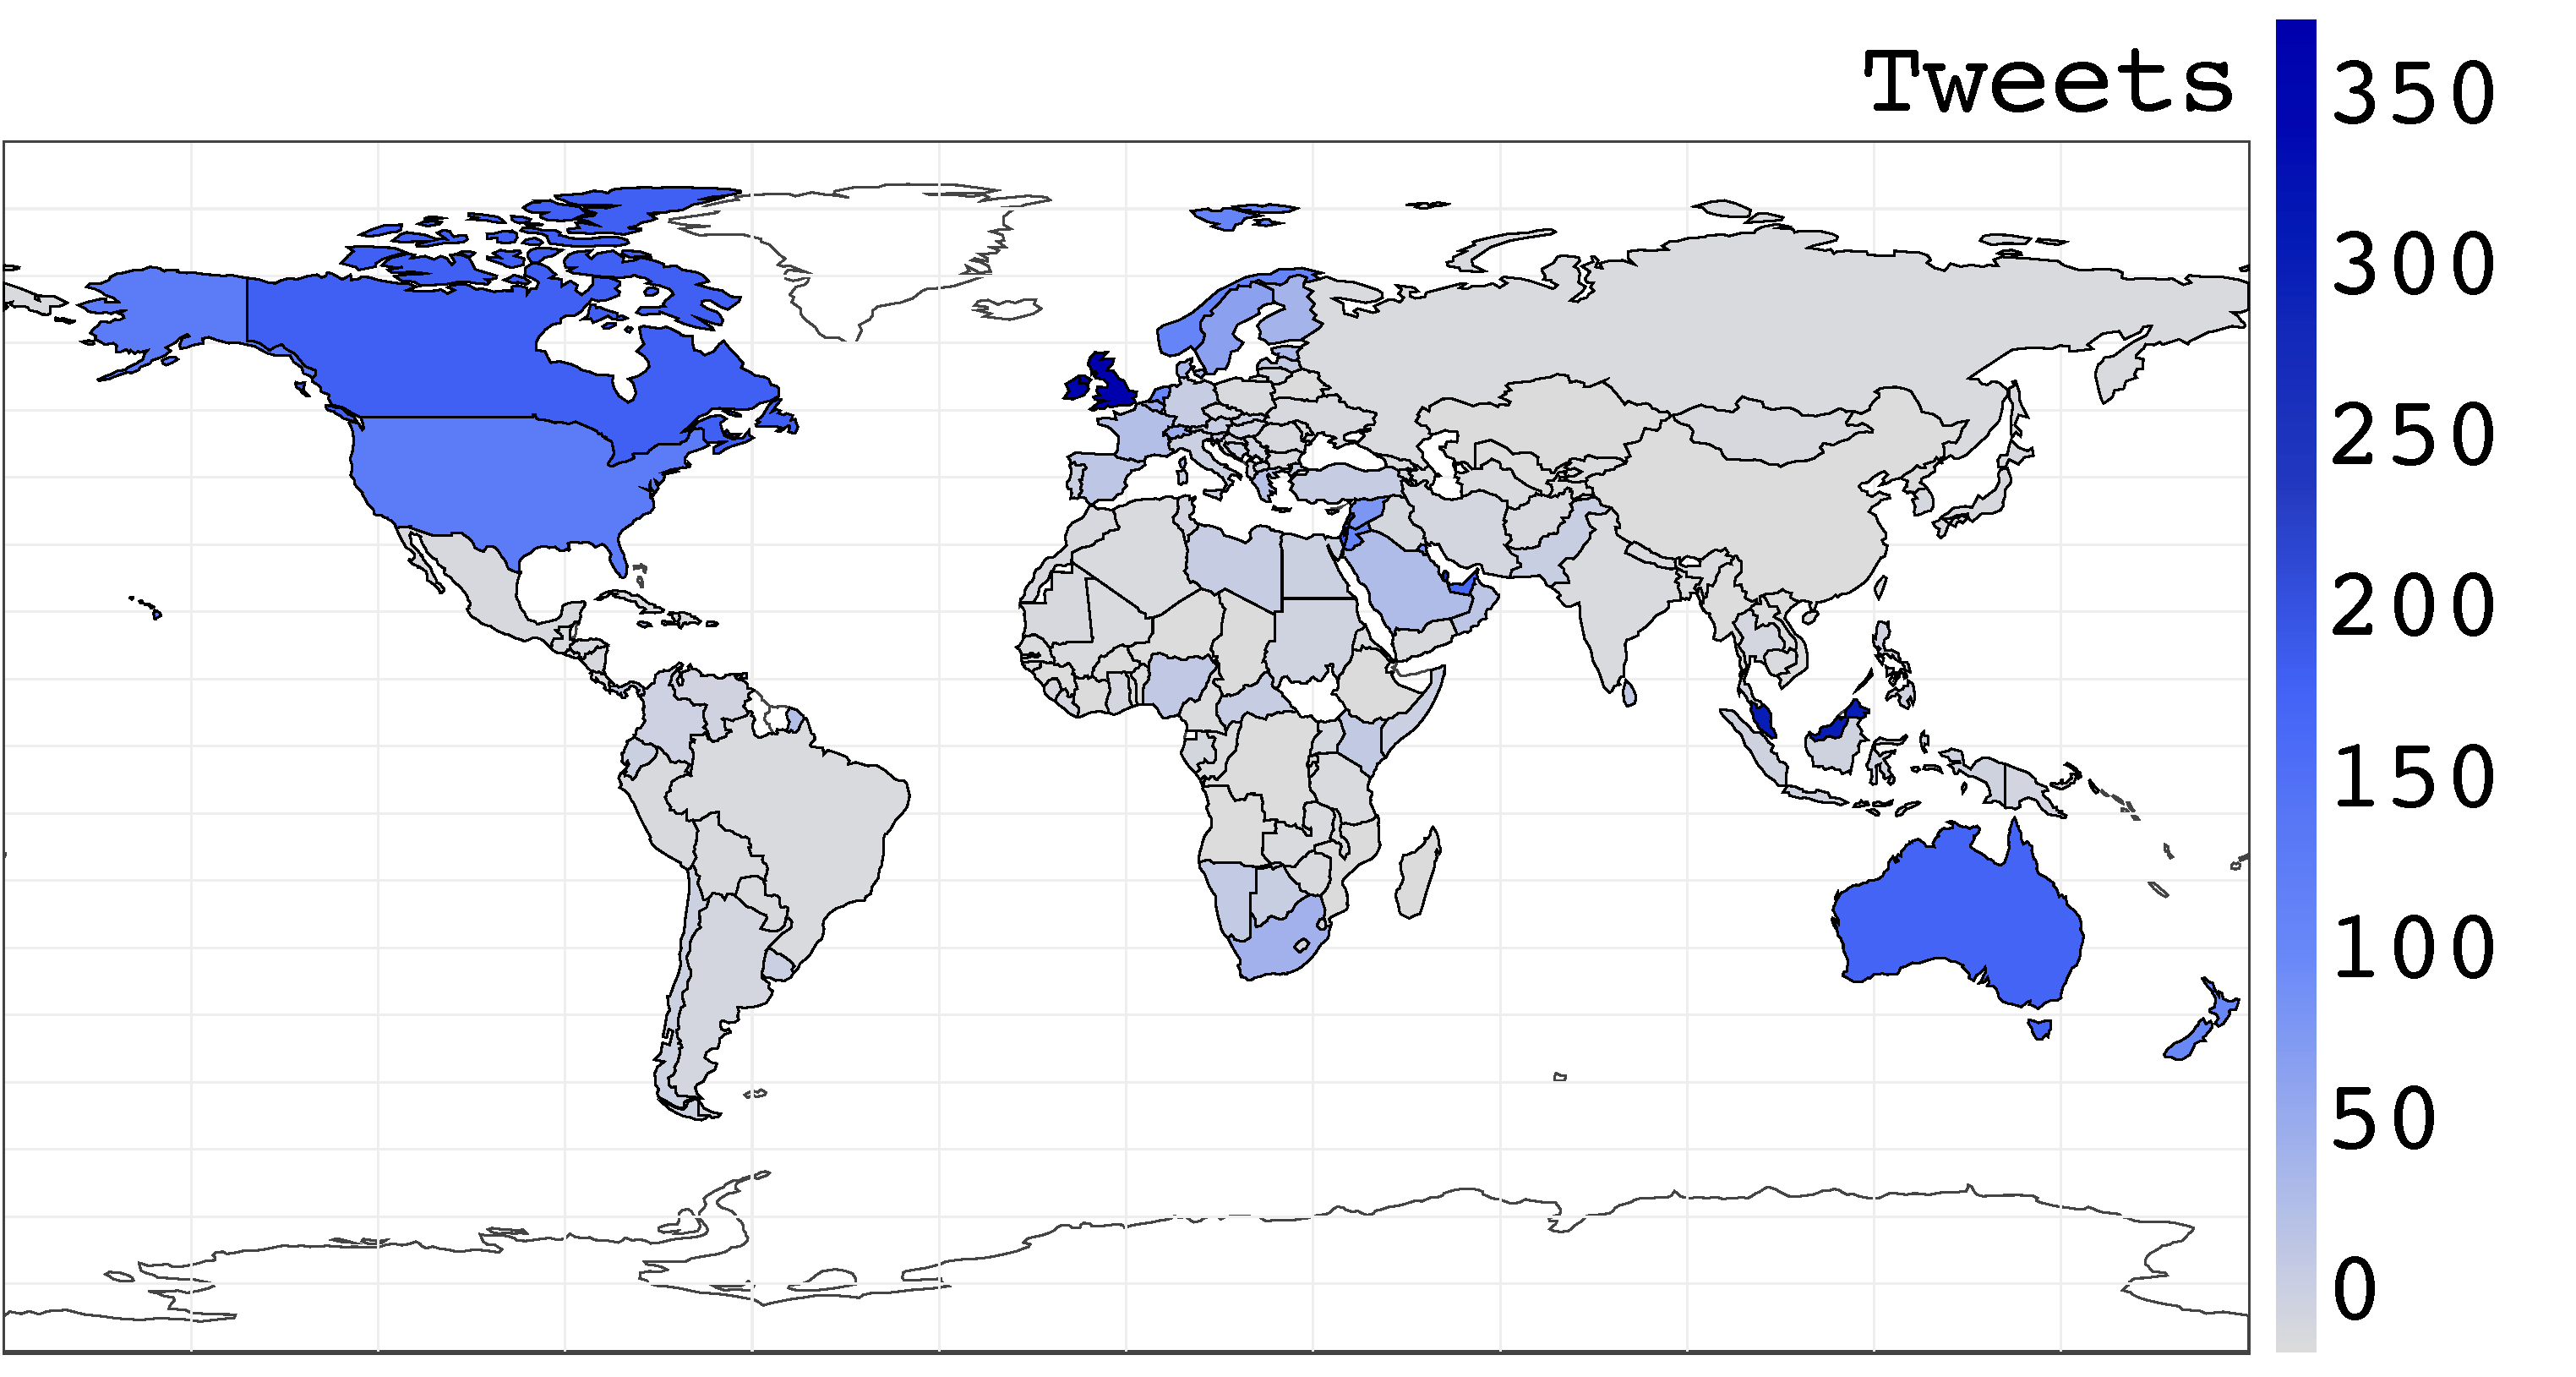
\includegraphics[width=0.33\textwidth]{images/location/world/socialsensor-world-humancauseddisaster_location.pdf}}
\subfloat[Fig:][Iran Deal]{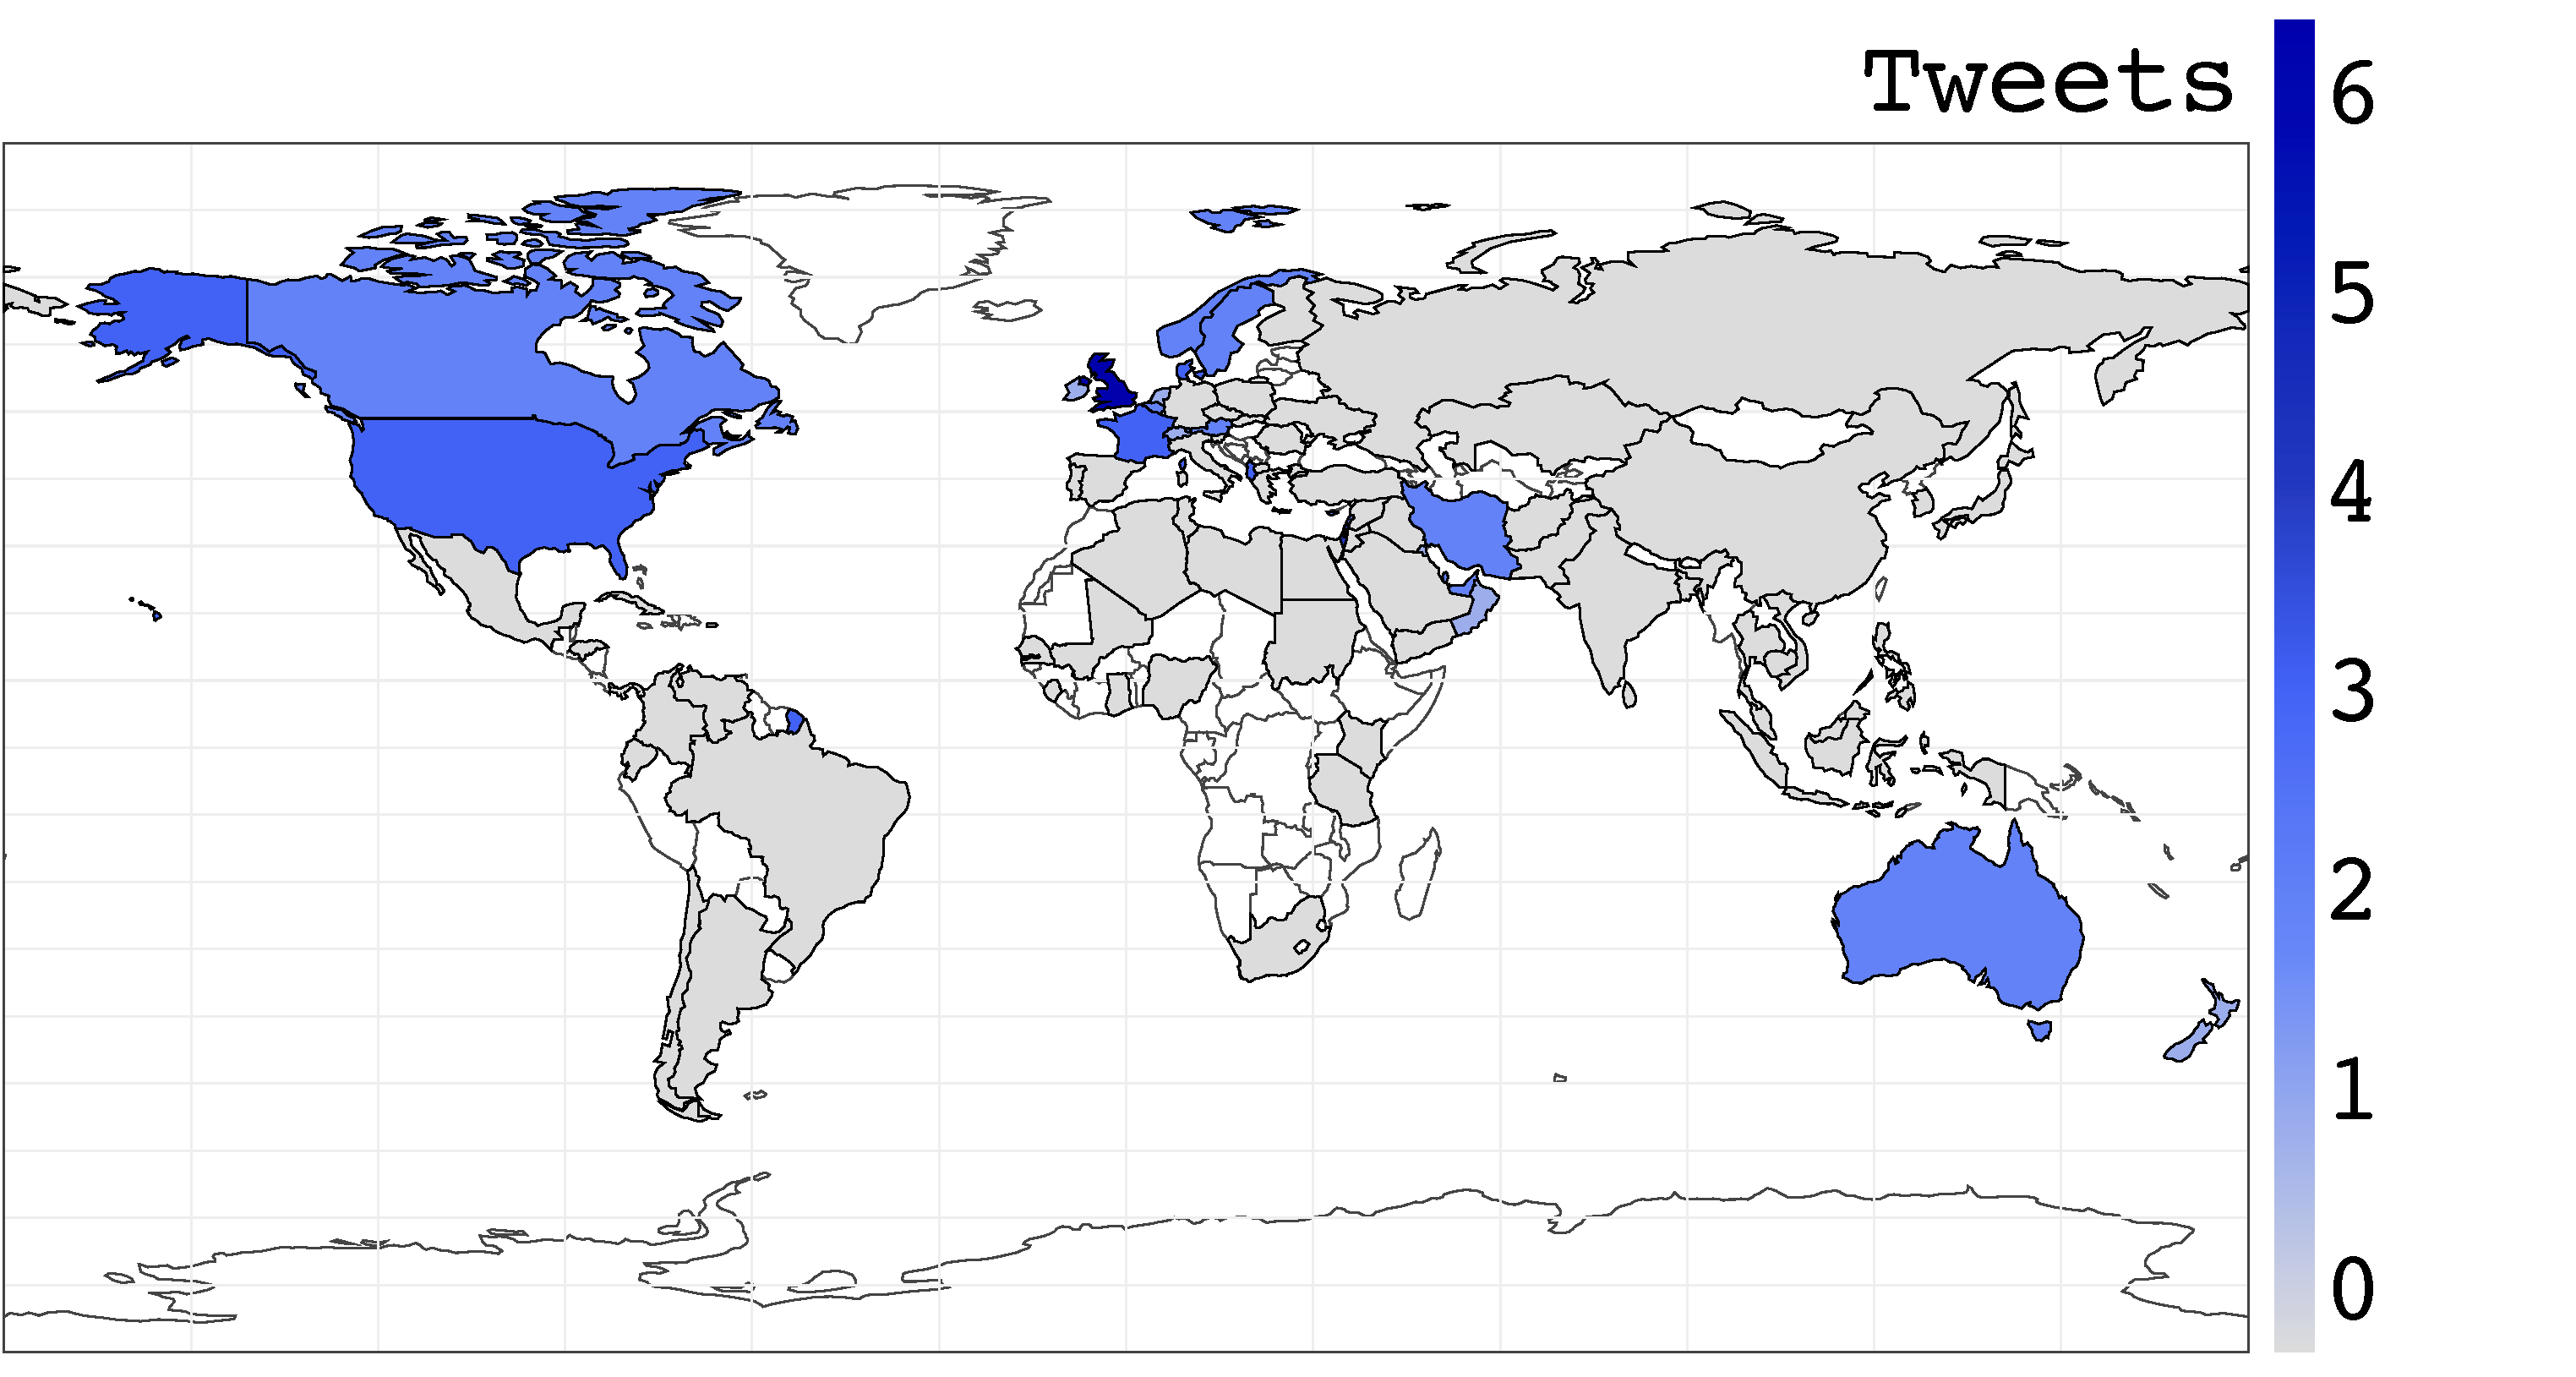
\includegraphics[width=0.33\textwidth]{images/location/world/socialsensor-world-irannucleardeal_location.pdf}}
\subfloat[Fig:][Soccer]{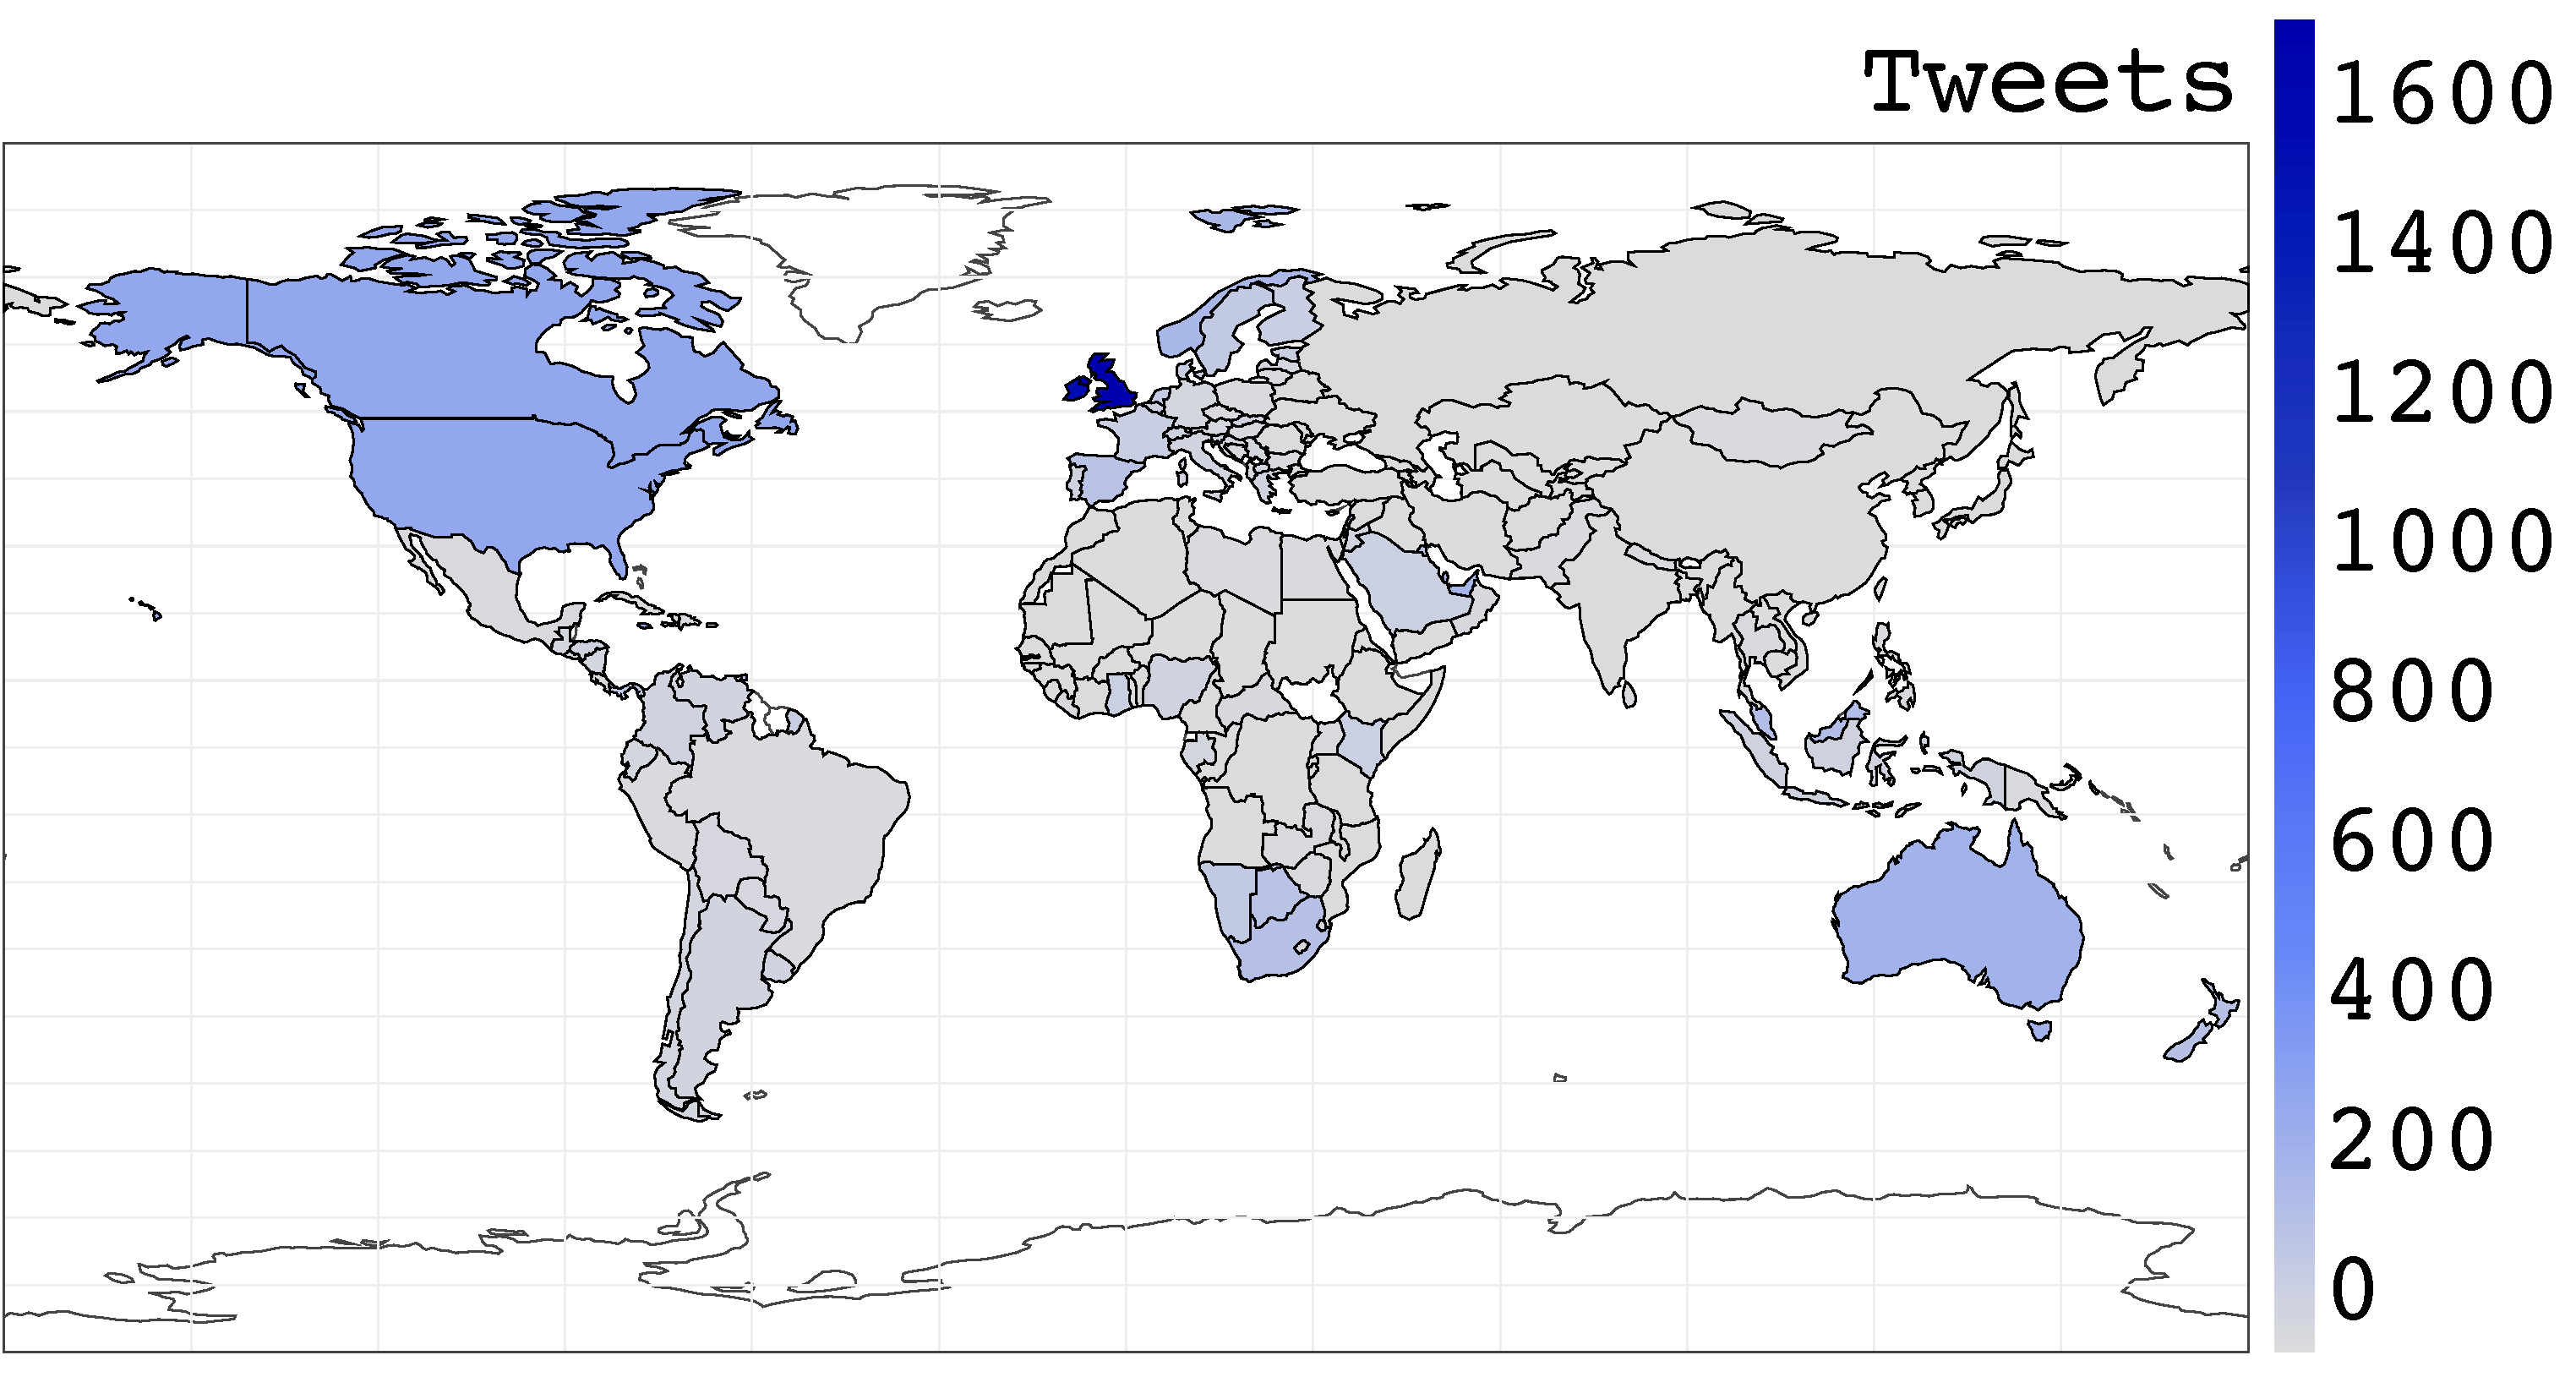
\includegraphics[width=0.33\textwidth]{images/location/world/socialsensor-world-soccer_location.pdf}} \\
%\vspace{-10mm}
\subfloat[Fig:][Health Epidemics]{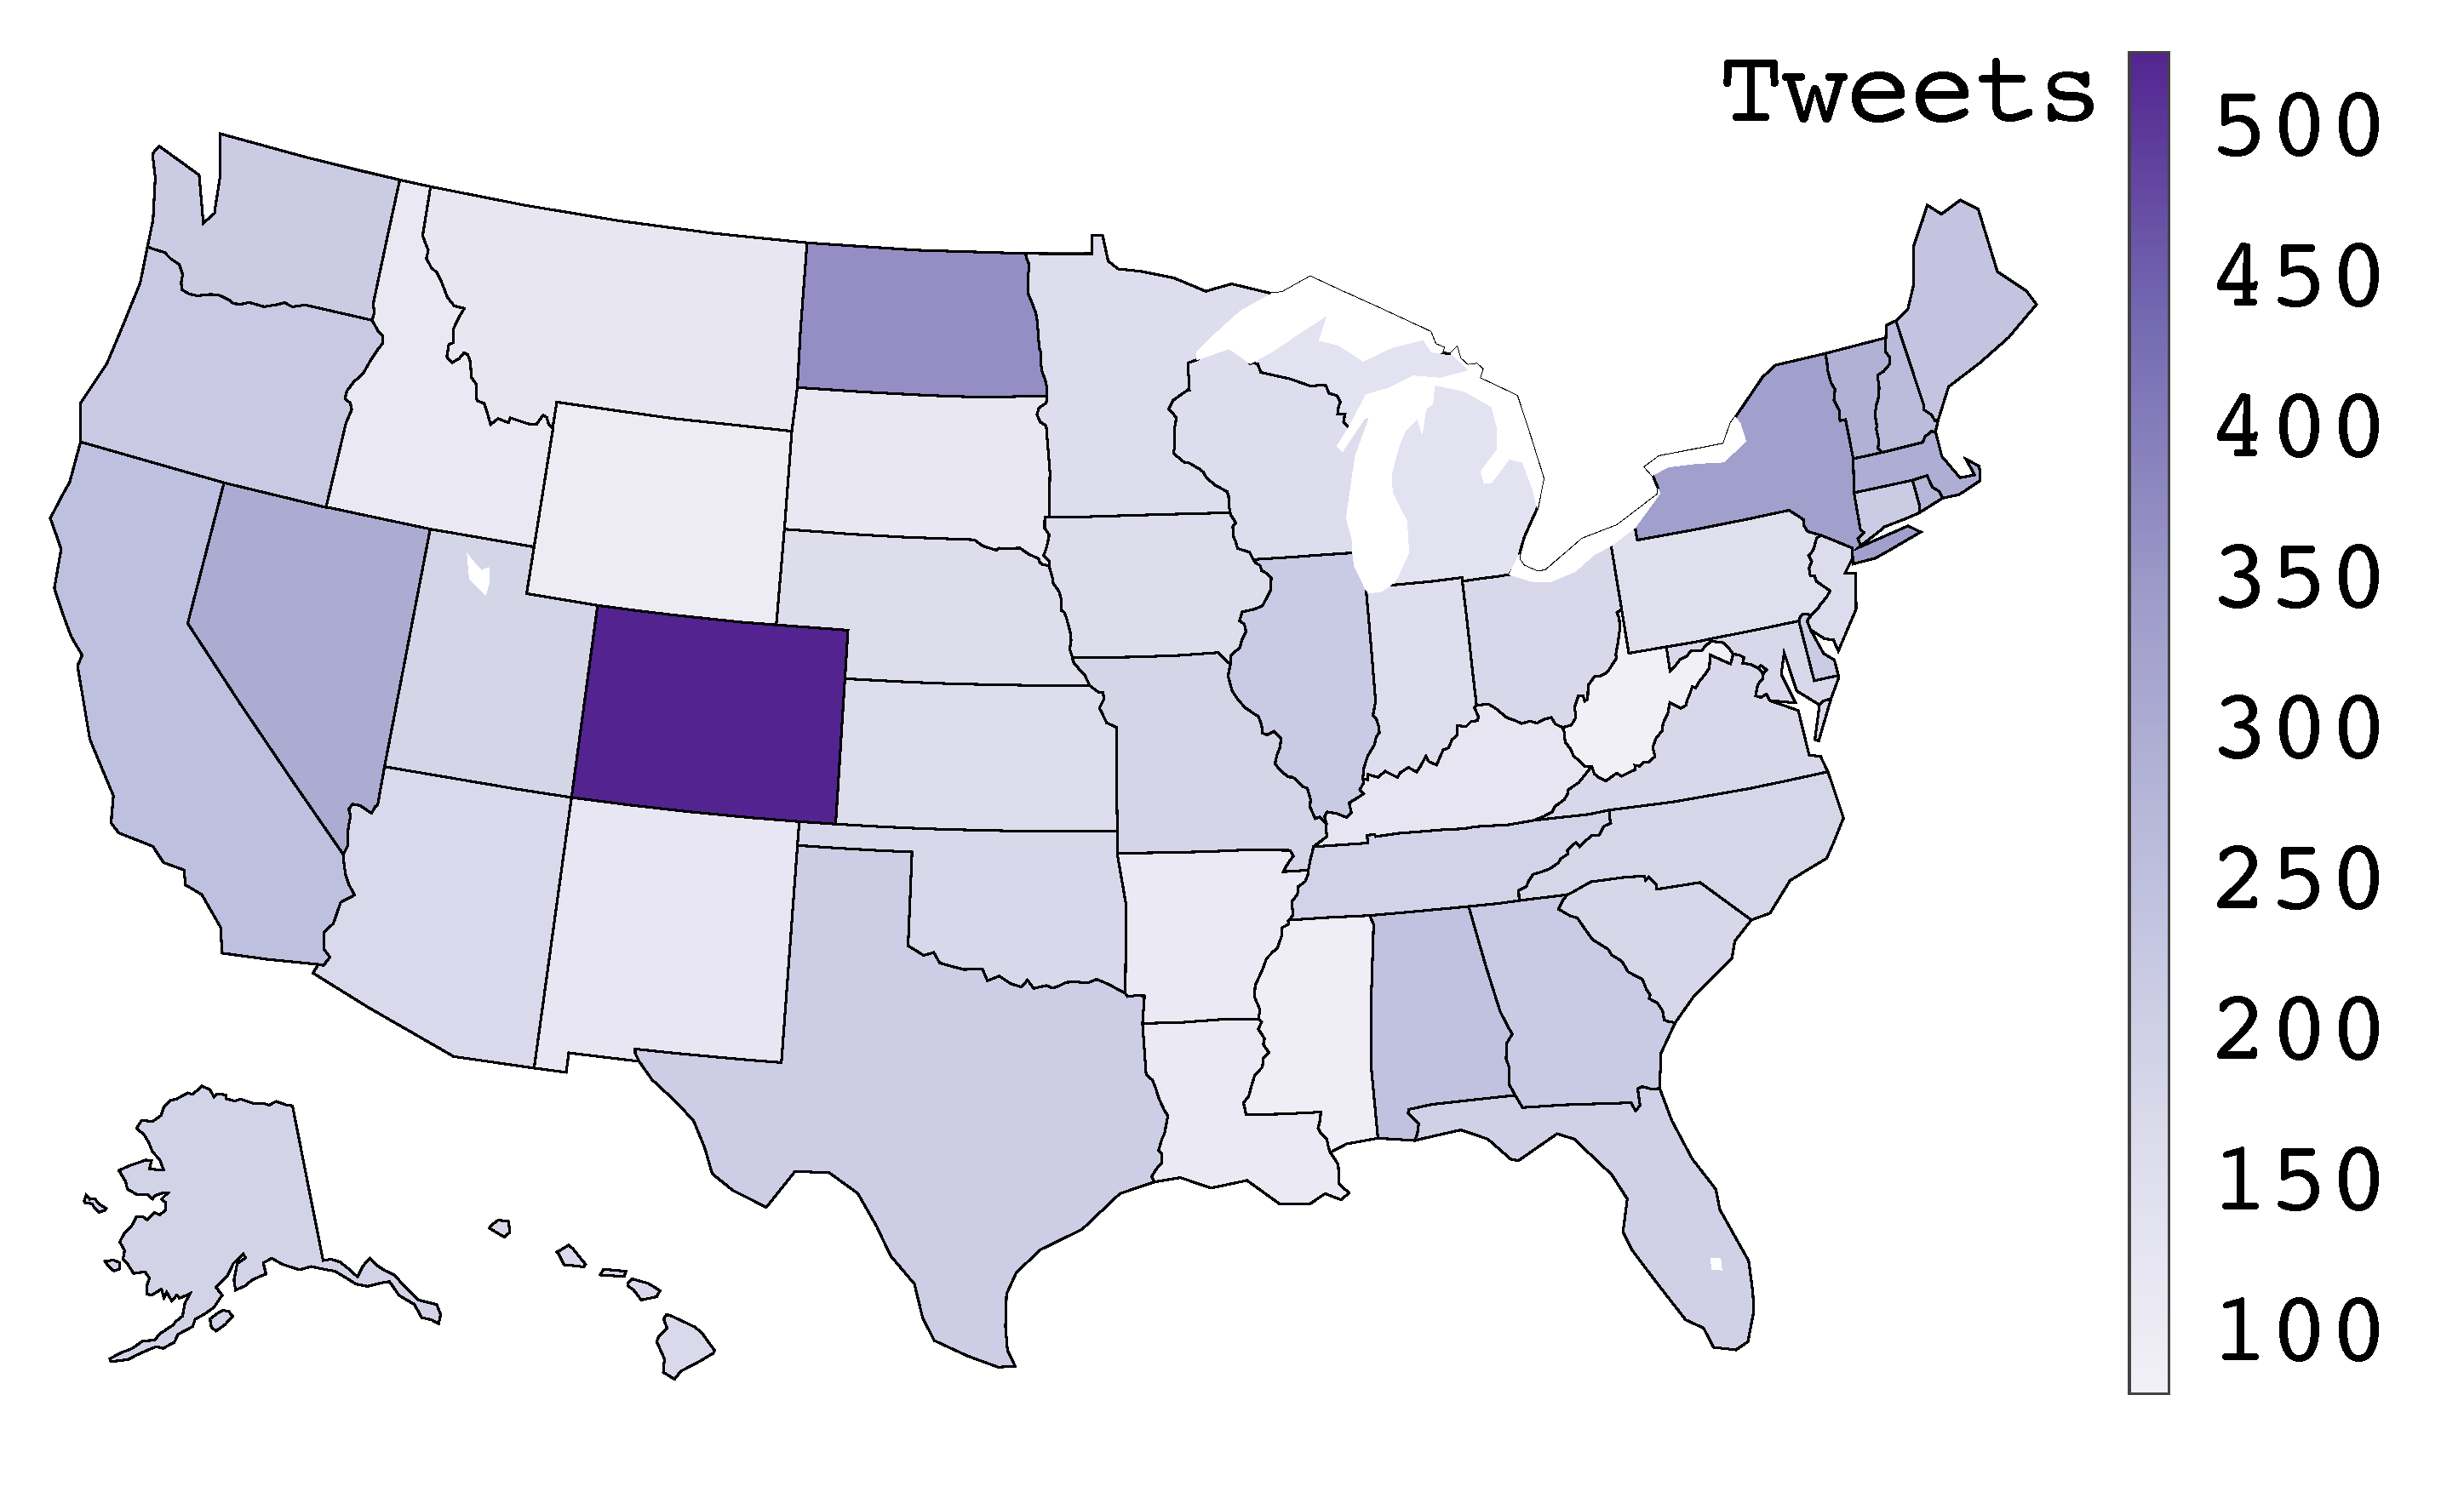
\includegraphics[width=0.33\textwidth]{images/location/states/SocialSensor-us-states-health_epidemics_location.pdf}}
\subfloat[Fig:][Social Issues]{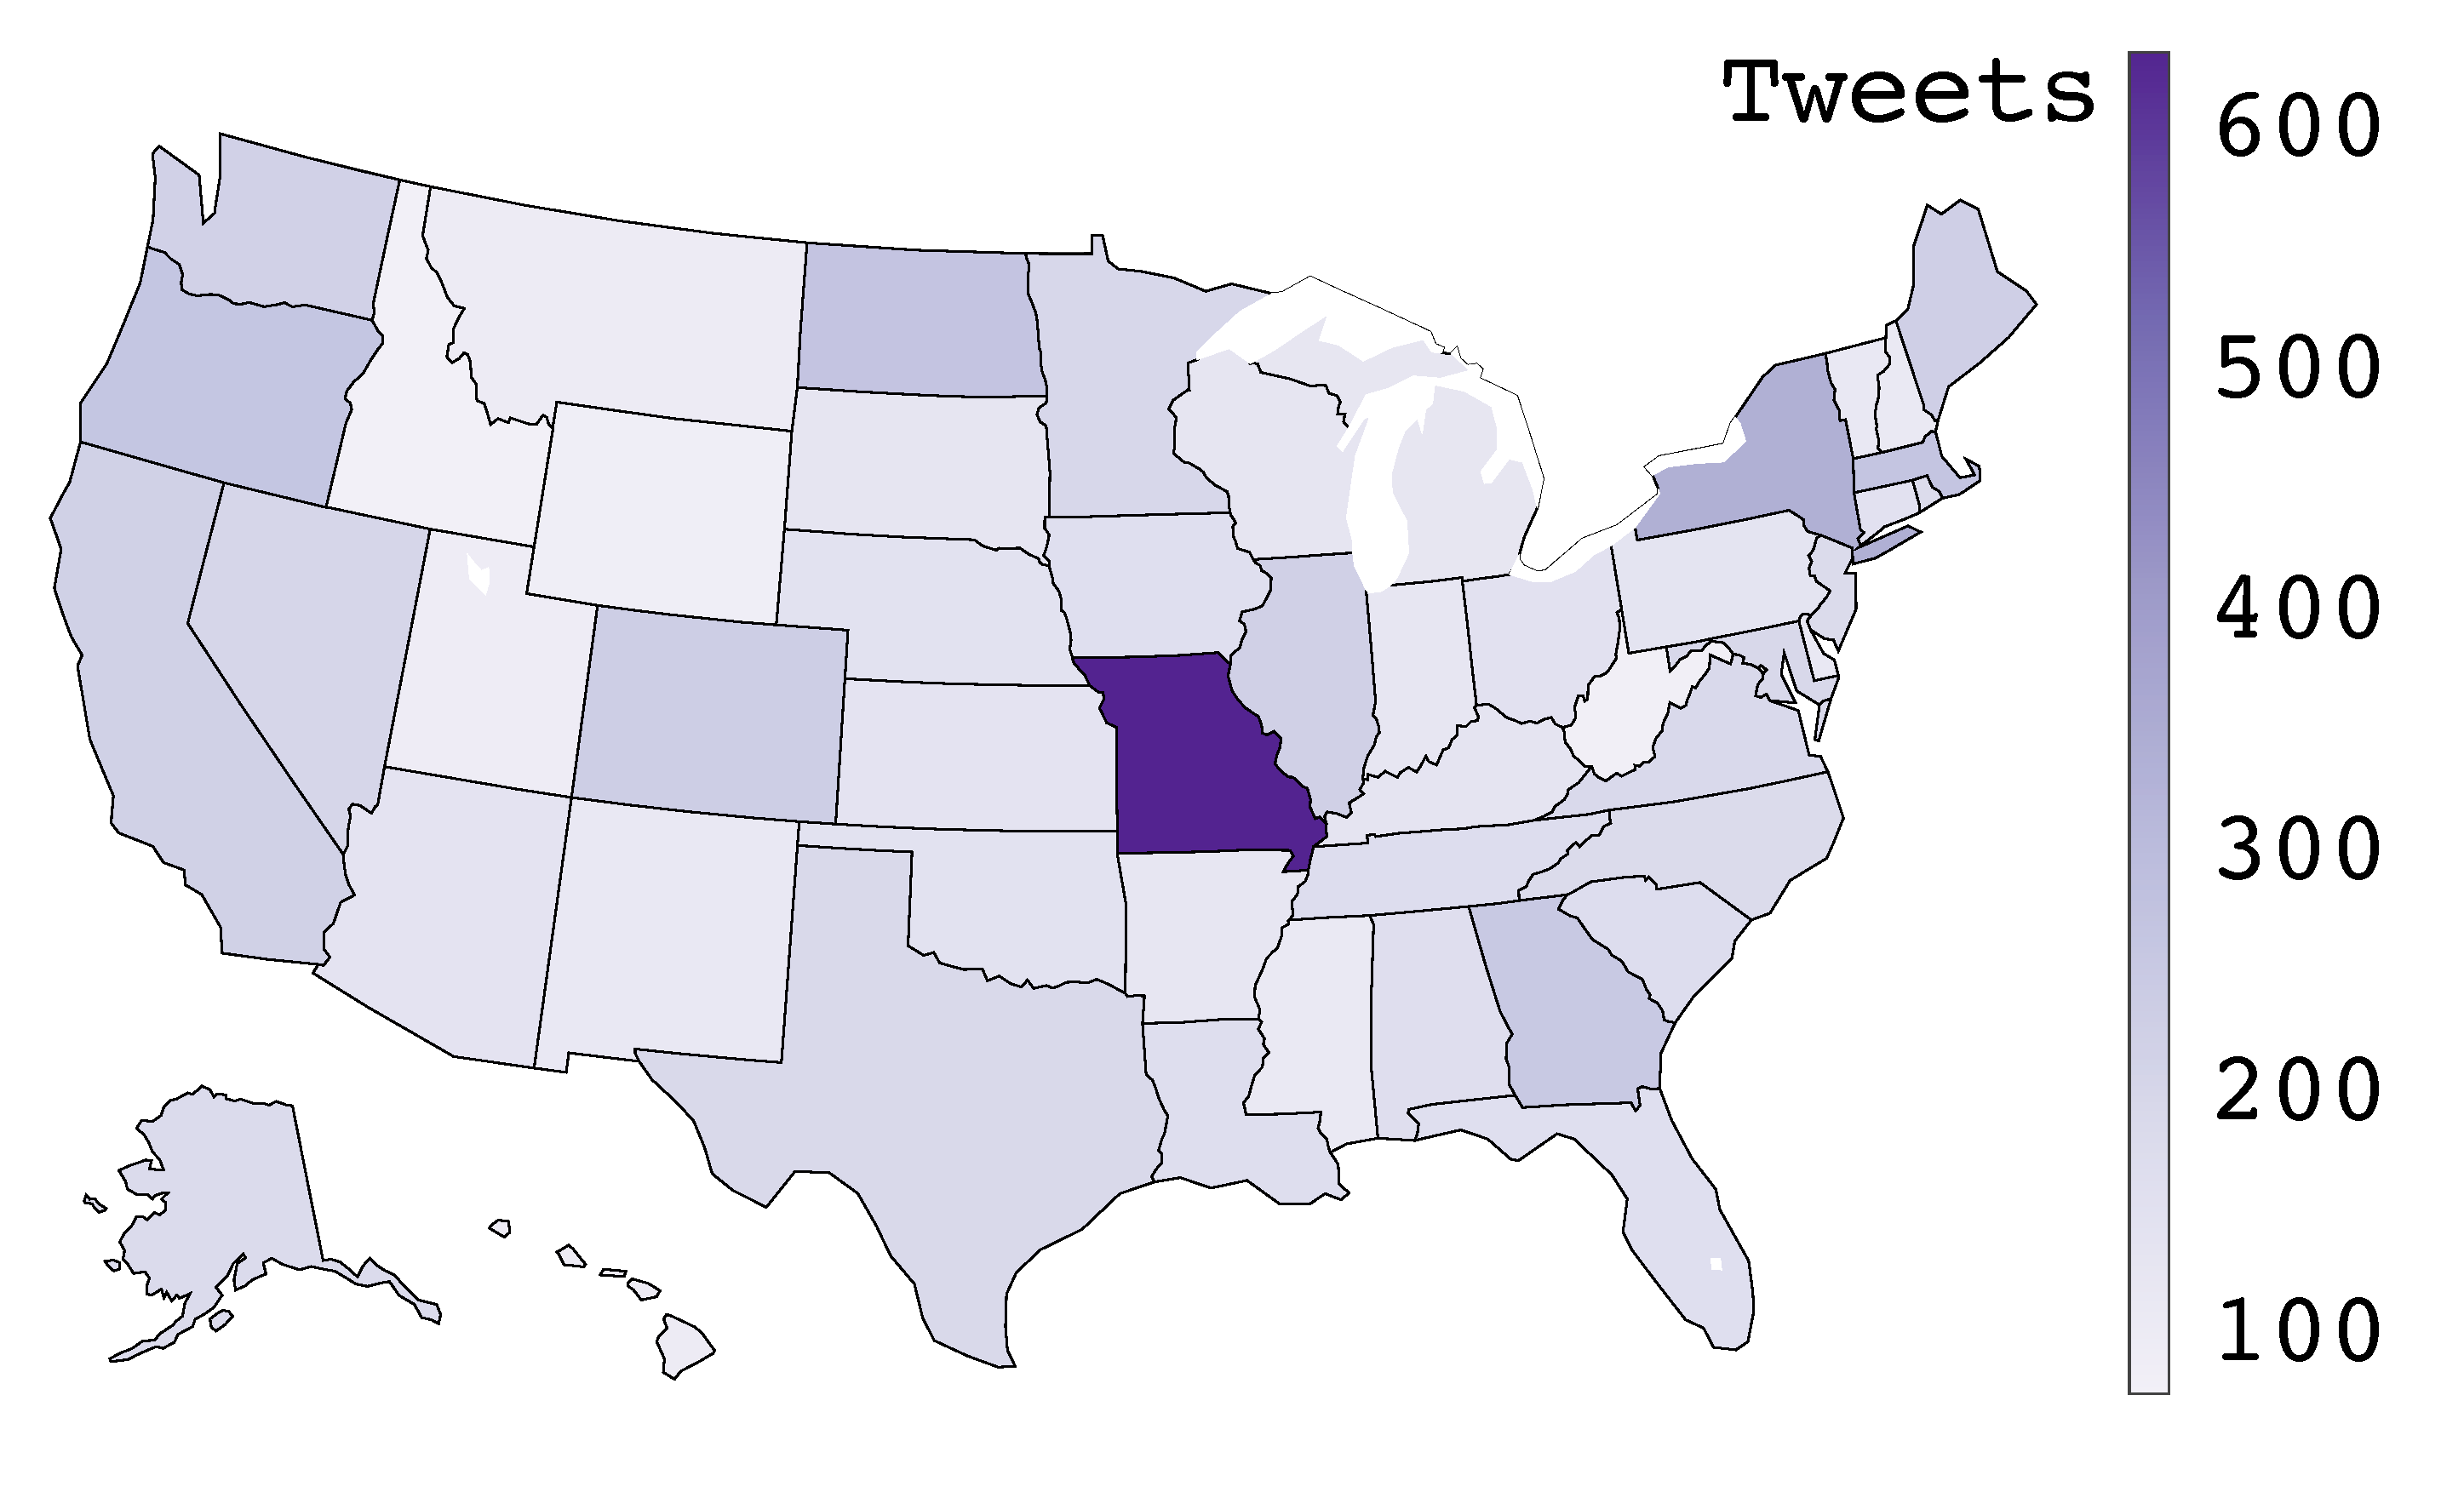
\includegraphics[width=0.33\textwidth]{images/location/states/SocialSensor-us-states-socialissues_location.pdf}}
\subfloat[Fig:][Space]{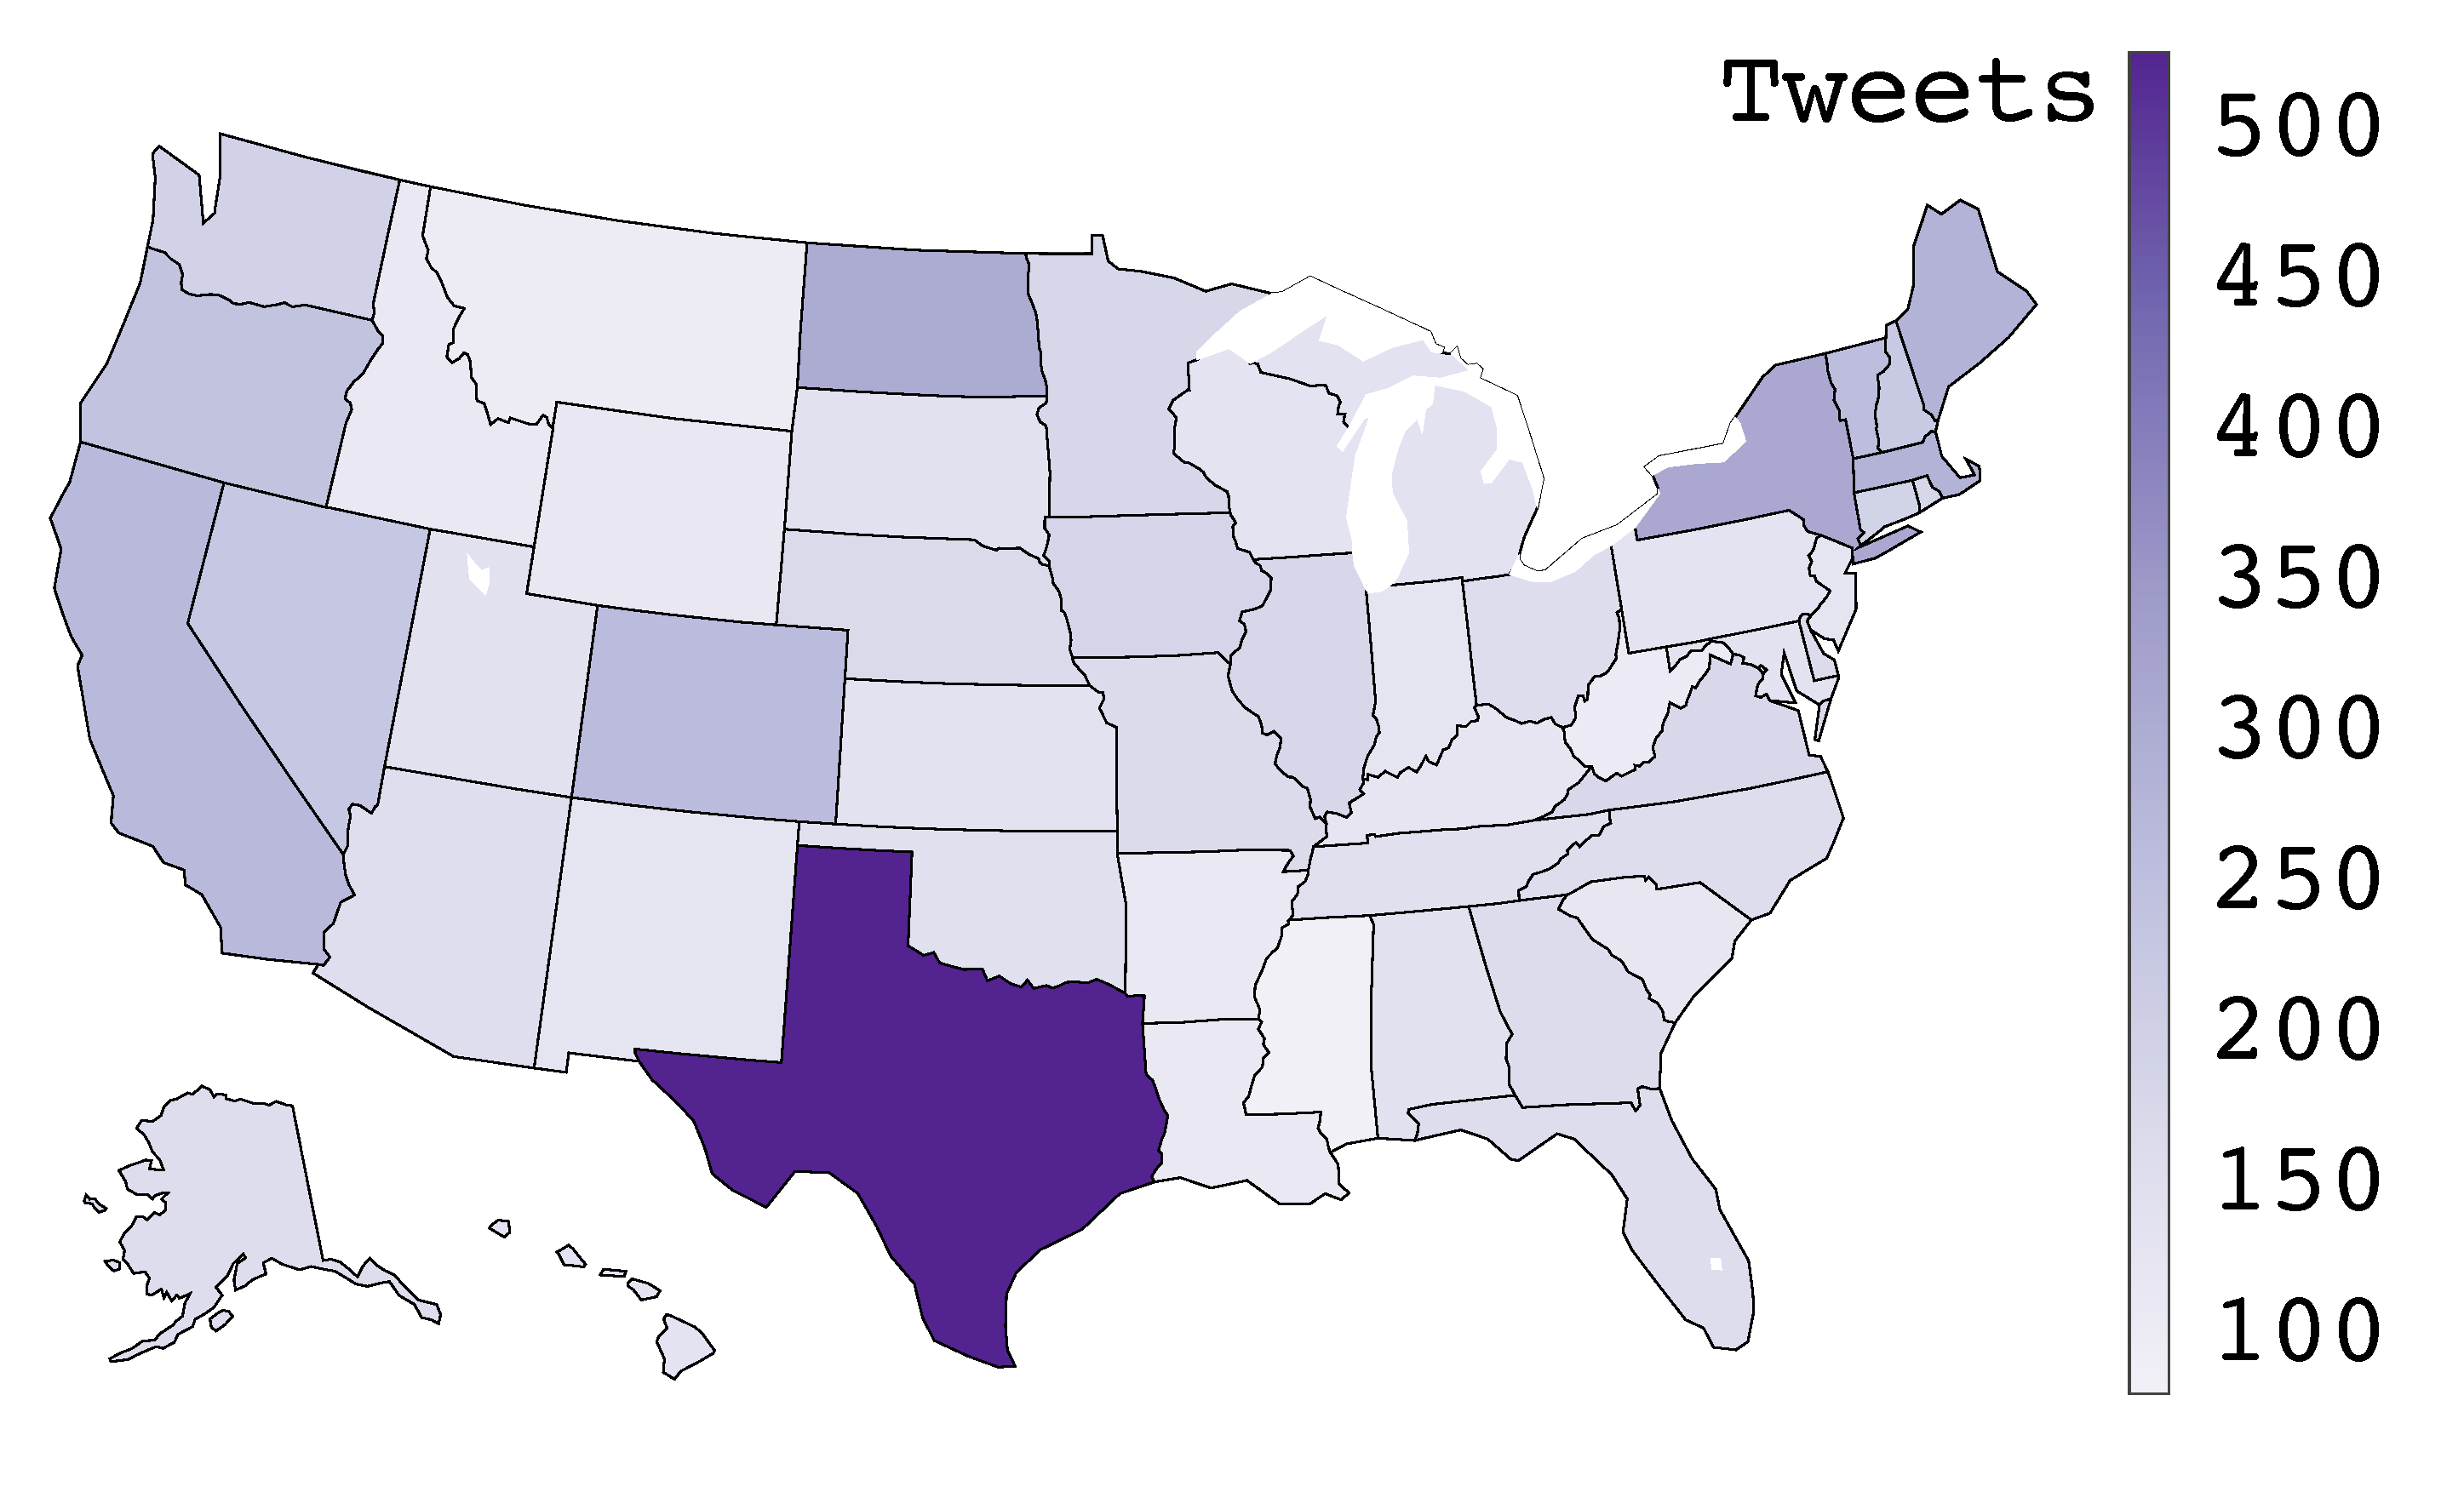
\includegraphics[width=0.33\textwidth]{images/location/states/SocialSensor-us-states-space_location.pdf}} \\
\end{tabular}
%\vspace{-2mm}
\caption {Per capita tweet frequency across different international and U.S. locations for different topics. The legend provides the number of tweets per 1 Million capita.}
\label{fig:choropleths}
\end{figure*}
%%%%%%%%%%%%%%%%%%%%%%%%%%%%%%%%%%%%%%%%%%%%%%%%%%%%%%%%%%%%%%%%%%%%%%%%%%%
%%%%%%%%%%%%%%%%%%%%%%%%%%%%%%%%%%%%%%%%%%%%%%%%%%%%%%%%%%%%%%%%%%
\begin{table}[t!]
\centering
\caption{\label{table:featureStatistics}Feature Statistics of our $829,026,458$ tweet corpus.} % in our Twitter dataset}
{\renewcommand{\arraystretch}{1.2}
\resizebox{0.48\textwidth}{!}{%
\begin{tabular}{|c|c|c|c|c|}
%\hline
\multicolumn{5}{c}{\textbf{\#Unique Features}} \\ \hline
\textbf{User} & \textbf{Hashtag} & \textbf{Mention} & \textbf{Location} & \textbf{Term} \\ \hline
95,547,198 & 11,183,410 & 411,341,569 & 58,601 & 20,234,728 \\ \hline %14,197,509
%\end{tabular}
%}}
%\vspace{.5mm}
%\caption{Number of unique features for each type.}%values for each feature of $829,026,458$ tweets in our Twitter dataset}
%\label{table:featureUnique}
%\end{table}
%
%\begin{table}[t!]
%\centering
%{\renewcommand{\arraystretch}{1.2}
%\resizebox{0.48\textwidth}{!}{%
%\begin{tabular}{|l|c|c|c|c|}
%\hline
\multicolumn{5}{c}{} \\
\multicolumn{5}{c}{\textbf{Feature Usage in \#Tweets}} \\ \hline
\textbf{Feature} & \textbf{Max} & \textbf{Avg} & \textbf{Median} & \textbf{Most frequent} \\ \hline
\textbf{User} & 10,196 & 8.67 & 2 & running\_status \\ \hline
\textbf{Hashtag} & 1,653,159 & 13.91 & 1 & \#retweet \\ \hline
\textbf{Mention} & 6,291 & 1.26 & 1 & tweet\_all\_time \\ \hline %$\rightarrow$null \\ \hline
\textbf{Location} & 10,848,224 & 9,562.34 & 130 & london \\ \hline
\textbf{Term} & 241,896,559 & 492.37 & 1 & rt \\ \hline 
\multicolumn{5}{c}{} \\
\multicolumn{5}{c}{\textbf{Feature Usage by \#Users}} \\ \hline
\textbf{Hashtag} & 592,363 & 10.08 & 1 & \#retweet \\ \hline
\textbf{Mention} & 26,293 & 5.44 & 1 & dimensionist \\ \hline
\textbf{Location} & 739,120 & 641.5 & 2 & london \\ \hline
\textbf{Term} & 1,799,385 & 6,616.65 & 1 & rt \\ \hline %SHOULD BE FIXED
\multicolumn{5}{c}{} \\
\multicolumn{5}{c}{\textbf{Feature Using \#Hashtags}} \\ \hline
\textbf{User} & 18,167 & 2 & 0 & daily\_astrodata \\ \hline
\textbf{Location} & 2,440,969 & 1,837.79 & 21 & uk \\ \hline
\end{tabular}
}}
\end{table}
%%%%%%%%%%%%%%%%%%%%%%%%%%%%%%%%%%%%%%%%%%%%%%%%%%%%%%%%%%%%%%%%%%

We begin with details of the Twitter testbed for topical classifier learning
that we evaluate in this paper.  We crawled Twitter data using Twitter
Streaming API for two years spanning 2013 and 2014 years.
%This type of crawling provides us with a very sparse set of data, roughly $1\%$ of all tweets \footnote{\hyperref[]{http://allthingsd.com/20101110/twitter-firehose-too-intense-take-a-sip-from-the-garden-hose-or-sample-the-spritzer|}}. 
We collected more than 2.5 TB of compressed data, which contains a total number 
of $829,026,458$ English tweets. In the context 
of Twitter, we consider five feature types for each tweet.  Each
tweet has a \textit{User} feature (i.e., the person who tweeted it), a
possible \textit{Location} (i.e., a string provided as meta-data), and
a time stamp when it was posted.  A tweet can also contain one or more
of the following:
\begin{itemize}
%NOTE: $$ is not for italics... it is for math mode and has larger math mode spacing
%since adjacent letters are implicitly multiplied.  Use \textit -SPS
\item \textit{Hashtag}: a topical keyword specified using the \# sign.
\item \textit{Mention}: a Twitter username reference using the @ sign. % reply?
\item \textit{Term}:    any non-hashtag and non-mention unigrams. %These uni-grams are later cleaned to remove $Term$s with no meaning (total number of $Term$s before cleaning was $20,234,729$)
\end{itemize}
We provide more detailed statistics about each feature in
Table~\ref{table:featureStatistics}.  For example, there are
over 11 million unique hashtags, the most frequent unique hashtag
occurred in over 1.6 million tweets,
a hashtag has been used on average by $10.08$ unique users, and 
authors (\textit{Users}) have used a median value of $2$
tweets. % not average, median!!! -SPS

Figure~\ref{fig:choropleths} shows per capita tweet frequency across
different international and U.S. locations for different topics.
While English speaking countries dominate English tweets, we see that
the Middle East and Malaysia additionally stand out for the topic of
Human Caused Disaster (MH370 incident), Iran, U.S., and Europe for nuclear
negotiations the ``Iran deal'', and soccer for some (English-speaking)
countries where it is popular.  For U.S. states, we see that Colorado
stands out for health epidemics (both whooping cough and pneumonic
plague), Missouri stands out for social issues (\#blacklivesmatter in
St. Louis), and Texas stands out for space due to NASA's presence
there.


\section*{Methodology}
\label{sec:methodology}
%!TEX root = main.tex

\textcolor{red}{In this section, we describe the formal framework we use for our longitudinal study of topic classification. Hence, we first describe how we propose to label the data using a set of hand-curated user hashtags. Then, we proceed to describe the way we propose to split the dataset into train, validation and test sets, which is critical for such a longitudinal study of topical classifiers. 
Finally, we provide a brief description of several classification algorithms we use in our analysis.
}

% =====================
% What are we doing?  
% (1) Formal problem setup and notation definitions.  Corpus of documents, features, labels, classification problem definition (for a generic classifier).
% (2) How we label data.
% (3) How we train (validation set critical for hyperparameters, what metric used for selection?).
% Note that formal performance evaluation provided in experimental section.
% =====================

% (1) Formal problem setup and notation definitions.  Corpus of documents, features, labels, classification problem definition (for a generic classifier).
%TODO: Formal learning framework.

  
%
%To this end, we now outline a methdology for training and evaluating such topic classifiers.
%
%{\color{red}
%In this section, we reduce the problem of learning topical content from large space of features and small set of examples provided by the user to the following setting that will match standard supervised learning paradigm.
%
%Here, the problem statement is that the user has an information need for high-precision topical content from Twitter. 
%The first step for the user is that he/she must provide labeled data to represent this information need for use in a targeted supervised learning setting.
% We assume that for each topic, the user will provide us with a set of hashtags. For example for the topic of \textit{Natural Disaster}, 
%the user will give us \{\#earthquake,\#flood,\#prayforthephilippines, ...\}. The goal is, given this topic and related hashtags, return a ranked
% list of tweets to the user that are highly relevant to the topic and match users information needs; meaning instead of returning a set of tweets
% that only match "disaster" or "natural", we realize the actual information need behind the searched topic and present all tweets matching this need. 
%To this end, we need a methodology that learns from the set of hashtags provided by users on how to pick up sensors (i.e., useful terms, mentions, 
%hashtags, locations, and users) and weight them to ensure picking new, unseen topical hashtags in future tweets. The following discussion intends
% to answer how to develop such methodology. 
%
%To this end, we assume a birth-time for each hashtag as the first time it has been used in our dataset. Assuming a birth-time, then we consider temporal split of our chosen set of hashtags and learn on one set and test on the other more recent set to evaluate the methods generalizability. The limitation of this method is since we use hashtags as topical proxies, we mislabel the tweets without hashtags. Therefore, we miss part of topical content that we could learn from for the price of automatic labeling of all tweets with minimal user effort. Now, we move on to mathematically formalize this problem.}
% }
% 

%In an ideal scenario, we could train for topic $t$ 
%so that $\forall d_i \; f^t(d_i) = t(d_i)$ --- our scoring
%function (or more generally some threshold on it yielding a $\{0,1\}$ prediction) agrees perfectly with the topic
%labels of all tweets.  

%There are two catches that make our training setting somewhat
%non-standard and which underlie key difficulties when training topical
%classifiers for Twitter:  (1) Manually labeling documents is time-consuming so
%we need a way to manually label a large number of tweets with minimal
%user curation effort; \emph{We achieve this by leveraging the insight of
%of~\cite{lin2011smoothing} and use a set of predefined hashtags as topical proxies.}
%(2) We need to train our social sensor on
%known topical content, but tune it on novel topical validation content 
%that ensures the tuning achieves optimal generalization; \emph{We achieve this by 
%excising training content from our validation data so that our scoring
%function hyperparameter tuning ensures generalization.}
%We elaborate on these details next.

%\begin{equation}
%(\gamma, M) : D \to T 
%\end{equation}
%\part{title}
%\begin{equation}
%t^{*} = argMin_{w} L(t,\hat{t})
%\end{equation}
%
%Where ${L : T \times T \to \Re_{+} }$ is the loss function indicating the penalty for an incorrect prediction and ${L(t,\hat{t})}$ is the loss for prediction of ${\hat{t}}$ instead of actual topic $t$.

%SCORING TWEETS AT TEST TIME
%Each document ${d_{i}} \in D$ is scored for a given topic ${t \in \{ T \}}$ by the measure of it's similarity to the topic defined as
%
%\begin{equation}
%Sim({d_{i}}, t) = \sum_{j} F_{d_{i}}^{j}) \times {w_{j}}
%\end{equation}
%
%where $F_{d_{i}}^{j}$ represents the $j$th value in $F_{d_{i}}$.

% (2) How we label data.

\subsection*{Dataset labelling}

A critical bottleneck for learning targeted topical social classifiers 
is to achieve sufficient supervised content labeling.  With data
requirements often in the thousands of labels to ensure effective
learning and generalization over a large candidate feature space (as
found in social media), manual labeling is simply too time-consuming
for many users, while crowdsourced labels are both costly and prone to
misinterpretation of users' information needs.  Fortuitously, hashtags
have emerged in recent years as a pervasive topical proxy on social
media sites --- hashtags originated on Internet Relay Chat (IRC), were adopted later
(and perhaps most famously) on Twitter, and now appear on other social
media platforms such as Instagram, Tumblr, and Facebook.  Following
the approach of~\cite{lin2011smoothing}, for each topic $t \in T$, we leverage a (small) set of
user hand-curated topical hashtags $H^t$ to efficiently label a large number of
supervised topic labels for social media content.  

Specifically, we manually curated a broad thematic range of 10 topics shown in the top row of
Table~\ref{table:sampleHashtags} by annotating hashtag sets $H^t$ for each topic $t \in T$.  
We used 4 independent annotators to query the Twitter search API to identify candidate hashtags for each topic, requiring an inner-annotator agreement of 3 annotators to permit a hashtag to be assigned to a topic set. 
\textcolor{red}{Samples of hashtags for each topic are given in the bottom row of Table~\ref{table:sampleHashtags}.}



\begin{table*}[t!]
\centering
\caption{Train/Validation/Test Hashtag samples and statistics.}
{\def\arraystretch{1.2}
\resizebox{\textwidth}{!}{%
% Preview source code for paragraph 0

% Preview source code for paragraph 0
% Preview source code for paragraph 0

\begin{tabular}{|c|c|c|c|c|c|c|c|c|c|c|}
\hline 
\multirow{2}{*}{} & \multirow{2}{*}{\textbf{Tennis}} & \multirow{2}{*}{\textbf{Space}} & \multirow{2}{*}{\textbf{Soccer}} & \textbf{Iran Nuclear} & \textbf{Human} & \textbf{Celebrity} & \textbf{Social} & \textbf{Natural} & \multirow{2}{*}{\textbf{Epidemics}} & \multirow{2}{*}{\textbf{LGBT}}\tabularnewline
 &  &  &  & \textbf{Deal} & \textbf{Disaster} & \textbf{Death} & \textbf{Issues} & \textbf{Disaster} &  & \tabularnewline
\hline 
\hline 
\textbf{\#TrainHashtags} & 62 & 112 & 144 & 12 & 57 & 33 & 37 & 61 & 55 & 30\tabularnewline
\hline 
\textbf{\#ValHashtags} & 14 & 32 & 42 & 2 & 8 & 4 & 5 & 4 & 17 & 9\tabularnewline
\hline 
\textbf{\#TestHashtags} & 14 & 17 & 21 & 3 & 12 & 7 & 8 & 17 & 13 & 5\tabularnewline
\hline 
\hline 
\textbf{\#+TrainTweets} & 21,716 & 5,333 & 14,006 & 6,077 & 153,612 & 155,121 & 27,423 & 46,432 & 14,177 & 1,344\tabularnewline
\hline 
\textbf{\#-TrainTweets} & 191,905 & 46,587 & 123,073 & 54,045 & 1,363,260 & 1,376,872 & 244,106 & 411,609 & 125,092 & 11,915\tabularnewline
\hline 
\hline 
\textbf{\#+ValTweets} & 884 & 2,281 & 4,073 & 1,261 & 53,340 & 23,710 & 3,088 & 843 & 4,348 & 50\tabularnewline
\hline 
\textbf{\#-ValTweets} & 7,860 & 20,368 & 36,341 & 11,363 & 473,791 & 210,484 & 27,598 & 7,456 & 39,042 & 443\tabularnewline
\hline 
\hline 
\textbf{\#+TestTweets} & 1,510 & 5,908 & 11,503 & 368 & 34,055 & 7,334 & 14,566 & 5,240 & 3,105 & 692\tabularnewline
\hline 
\textbf{\#-TestTweets} & 13,746 & 53,348 & 103,496 & 3,256 & 305,662 & 65,615 & 130,118 & 47,208 & 27,828 & 6,325\tabularnewline
\hline 
\hline 
 & \#usopenchampion & \#asteroids & \#worldcup & \#irandeal & \#gazaunderattack & \#robinwilliams & \#policebrutality & \#earthquake & \#ebola & \#loveislove\tabularnewline
\cline{2-11} \cline{3-11} \cline{4-11} \cline{5-11} \cline{6-11} \cline{7-11} \cline{8-11} \cline{9-11} \cline{10-11} \cline{11-11} 
\textbf{Sample} & \#novakdjokovic & \#astronauts & \#lovesoccer & \#iranfreedom & \#childrenofsyria & \#ripmandela & \#michaelbrown & \#storm & \#virus & \#gaypride\tabularnewline
\cline{2-11} \cline{3-11} \cline{4-11} \cline{5-11} \cline{6-11} \cline{7-11} \cline{8-11} \cline{9-11} \cline{10-11} \cline{11-11} 
\textbf{Hashtags} & \#wimbledon & \#satellite & \#fifa & \#irantalk & \#iraqwar & \#ripjoanrivers & \#justice4all & \#tsunami & \#vaccine & \#uniteblue\tabularnewline
\cline{2-11} \cline{3-11} \cline{4-11} \cline{5-11} \cline{6-11} \cline{7-11} \cline{8-11} \cline{9-11} \cline{10-11} \cline{11-11} 
 & \#womenstennis & \#spacecraft & \#realmadrid & \#rouhani & \#bombthreat & \#mandela & \#freetheweed & \#abfloods & \#chickenpox & \#homo\tabularnewline
\cline{2-11} \cline{3-11} \cline{4-11} \cline{5-11} \cline{6-11} \cline{7-11} \cline{8-11} \cline{9-11} \cline{10-11} \cline{11-11} 
 & \#tennisnews & \#telescope & \#beckham & \#nuclearpower & \#isis & \#paulwalker & \#newnjgunlaw & \#hurricanekatrina & \#theplague & \#gaymarriage\tabularnewline
\hline 
\end{tabular}

}
}
\label{table:sampleHashtags}
\end{table*}


\subsection*{Dataset splitting}


We now provide a procedure for labeling data with $H^t$ for training, validation and test.
Following this, we proceed to train supervised classification and ranking methods to learn topical content from a large feature space -- this feature space includes terms, hashtags, mentions, authors and their locations. \textcolor{red}{ In the following, we describe three key points related to the temporal splitting of the dataset, sampling negative examples, and hyper-parameter tuning.}


%TODO: An simple enumeration of the training steps?
 \subfour{Temporally split for train, validation and test using $H^t$:}
As standard for machine learning methods, we divide our training data into
train, validation, and test sets --- the validation set is used for hyperparameter tuning to control
overfitting and ensure generalization to unseen data.  
As a critical insight for topical generalization where we view correct classification 
of tweets with \emph{previously unseen topical hashtags} as a proxy for topical generalization, 
we do not simply
split our data temporally into train and test sets and label both with \emph{all} 
hashtags in $H^t$. \textcolor{red}{ Rather,
we split each $H^t$ into three disjoint sets $H^t_\mathrm{train}$, $H^t_\mathrm{val}$, and $H^t_\mathrm{test}$
according to two time stamps $t^\mathrm{train}_\mathrm{split}$ and $t^\mathrm{val}_\mathrm{split}$ for topic $t$ and the first usage time stamp 
$h_\mathrm{time*}$ of each hashtag $h \in H^t$.  In short, all hashtags $h \in H^t$ first used
before $t^\mathrm{train}_\mathrm{split}$ are used to generate positive labels in the training data, all hashtags $h \in H^t$ first used
after $t^\mathrm{train}_\mathrm{split}$ and before $t^\mathrm{val}_\mathrm{split}$ 
are used to generate positive labels in the validation data,  and
the remaining hashtags are used to generate positive labels in the test data.}

\noindent To achieve this effect formally, we define the following:

\[
\begin{array}{l}
H_{\mathrm{train}}^{t}=\{h|h\in H^{t}\land h_{\mathrm{time*}}<t_{\mathrm{split}}^{\mathrm{train}}\}\\
H_{\mathrm{val}}^{t}=\{h|h\in H^{t}\land h_{\mathrm{time*}}\geq t_{\mathrm{split}}^{\mathrm{train}}\land h_{\mathrm{time*}}<t_{\mathrm{split}}^{\mathrm{val}}\}\\
H_{\mathrm{test}}^{t}=\{h|h\in H^{t}\land h_{\mathrm{time*}}\geq t_{\mathrm{split}}^{\mathrm{val}}\}
\end{array}
\]


Once we have split our hashtags into training and validation sets
according to $t^\mathrm{train}_\mathrm{split}$ and $t^\mathrm{val}_\mathrm{split}$, we next proceed to temporally split
our training documents $D$ into a training set $D^t_\mathrm{train}$, a validation set
$D^t_\mathrm{val}$, and a test set $D^t_\mathrm{test}$ for topic $t$ based on the posting
time stamp $d_{i,\mathrm{time*}}$ of each tweet $d_i$ as follows: 
%ormally, given $H^t$, we
%can label each document $d_i$ (containing positive features $D_i^+$) as follows:

% Preview source code for paragraph 0

\[
\begin{array}{l}
D_{\mathrm{train}}^{t}=\{d_{i}|d_{i}\in D\land d_{i,\mathrm{time*}}<t_{\mathrm{split}}^{\mathrm{train}}\}\\
D_{\mathrm{val}}^{t}=\{d_{i}|d_{i}\in D\land d_{i,\mathrm{time*}}\geq t_{\mathrm{split}}^{\mathrm{train}}\land d_{i,\mathrm{time*}}<t_{\mathrm{split}}^{\mathrm{val}}\land(\forall h\in d_{i}:h\notin H_{\mathrm{train}}^{t})\}\\
D_{\mathrm{test}}^{t}=\{d_{i}|d_{i}\in D\land d_{i,\mathrm{time*}}\geq t_{\mathrm{val}}^{\mathrm{train}}\land(\forall h\in d_{i}:h\notin H_{\mathrm{train}}^{t})\}
\end{array}
\]




The critical insight here is that we do not only divide the train, validation, and test
temporally, but we also divide the hashtag labels temporally and label the validation and test
data with an entirely disjoint set of topical labels from the training data. \textcolor{red}{Moreover, in order to avoid overfitting and allow a better generalization, we argue that removing tweets containing training hashtags is essential to avoid training a classifier that simply memorizes training hashtags. This latter proposal is experimentally evaluated later against a baseline where we simply keep all tweets containing training hashtags in the validation set.}
 



%\textcolor{red}{Next we define the set of positive tweet examples formally as} $D_i^+$ and note that
%$D_i^+$ may include feature IDs for the content of $d_i$ (e.g., terms and, importantly, 
%hashtags) as well as its meta-data (e.g., author, location).
Finally, to label the train, validation, and test data sets $D^t_\mathrm{train}$, $D^t_\mathrm{val}$ and $D^t_\mathrm{test}$, 
we use the respective
hashtag sets $H^t_\mathrm{train}$, $H^t_\mathrm{val}$, $H^t_\mathrm{test}$ for generating
the topic label for a particular tweet $t(d_{i}) \in \{0,1\}$ as follows:
\begin{align*}
t(d_{i}) & =
  \begin{cases}
    1 \textrm{ if }  \exists \; h \in d_i:  h  \in H^t  \\
    0  \textrm{ otherwise}
  \end{cases} .
\end{align*}
%To recap the methodology, we specify a set of hashtags as a proxy for a topic.  We split
%those hashtags into train and validation sets according to a time of first usage and fixed time point.
%We split the tweet data into train and validation sets according to the same fixed time point.
%Finally, we label a tweet in the train (validation) data set as positive if it contains
%a hashtag in the train (validation) hashtag set.  




The purpose behind this training, validation and test data split
and labeling is to ensure that learning hyper-parameters are tuned so as
to prevent overfitting and maximize generalization to unseen topical
content (i.e., new hashtags).
We remark that \emph{a classifier that simply
memorizes training hashtags will fail to correctly classify the validation data} except in 
cases where a tweet contains both a training and validation hashtag. 

Per topic, hashtags were split into train and test sets
according to their first usage time stamp roughly according to a 3/5
to 2/5 proportion (the test interval spanned between 9-14 months).  
The train set was further temporally subdivided
into train and validation hashtag sets according to a 5/6 to 1/6
proportion.  We show a variety of statistics and five sample hashtags
per topic in Table~\ref{table:sampleHashtags}.  Here we can see that
different topics had varying prevalence in the data
with \textit{Soccer} being the most tweeted topic
and \textit{Iran Nuclear Deal} being the least tweeted according to our curated
hashtags.


\subfour{Sampling negative examples:} \textcolor{red}{ Topic classification is very often considered as an unbalanced classification task since usually, there are much more negative examples than positive examples. Indeed, the large number of users on Twitter, their diversity, their wide range interests, and the short lifetime of topics discussed on a daily basis make that each topic has only a small set of positive examples.  For example, the Open Directory Project (ODP also known as DMOZ) provides a hierarchical classification structure of roughly 5M Web resources over 1M topics\footnote{http://www.geniac.net/odp/} -- each topic contains roughly 5 documents. Therefore, given the huge amount of negative examples in a real classification scenario (e.g., roughly 800 million negative examples against 500k positive examples for the human disaster topic), to efficiently tune each classifier, we have chosen to sample negative examples such that positive examples represent 10\% of the dataset and the negative examples represent 90\% of the dataset. This rule is valid for the training, validation and test sets of each topic.
 Details are provided in Table~\ref{table:sampleHashtags}.}




\subfour {Training and hyper-parameter tuning:}
Once $D^t_\mathrm{train}$ and $D^t_\mathrm{val}$ have been constructed,
we proceed to train our scoring function $f^t$ on $D^t_\mathrm{train}$ and
select hyperparameters to optimize Average Precision (AP) (a ranking
metric~\cite{manning_ir}) on
$D^t_\mathrm{val}$.  Once the optimal $f^t$ is found for $D^t_\mathrm{val}$,
we return it as our final learned topical scoring function $f^t$ for topic $t$.
Because $f^t(d_i) \in \mathbb{R}$ is a scoring function, it can be used to rank.
%\item {\bf Learning: The weight vector $W$ is learned with classification method $M$ on the selected set of documents using tuned hyper parameters
% Note that formal performance evaluation provided in experimental section.

%Analogously to train and validation data, test data is generated the same way.
%, but we omit formal notation (identical to the above) in order to reduce clutter.
%Test data has its own time stamp ($> t_\mathrm{split}$), its own set of
%temporally disjoint data, and its own set of hashtags 
%temporally disjoint from the training and validation data; this is done in order to evaluate
%generalization performance of the learned classifier on future data with topical hashtags
%not seen during training.    
With train, validation, and testing data defined along with the training methodology,
it remains now to extract relevant features, 
described next.









%%%%%%%%%%%%%%%%%%%%%%%%%%%%%%%%%%%%%%%%%%%%%%%%%%%%%%%%%%%%%%%%%%

%How we curated hashtags: need a good story here.  Inner-annotator agreement of 3/4.
% With the formal definition of learning topical classifiers provided
% in Sec.~\hyperref[sec:lss]{Learning Topical Social Sensors} and the overview of our data in
% Sec.~\hyperref[sec:datasetStatistics]{Data Description}, we proceed to outline our
% experimental methodology on our Twitter corpus.  
 
%As noted in Sec.~\hyperref[sec:datasetStatistics]{Data Description},

\subsection*{Topic classification features}

\textcolor{red}{The set of features that we consider for each tweet $d_i$ are: (i) \textit{User} (author of the tweet), (ii) \textit{Mention}, (iii) \textit{Location}, (iv) \textit{Term}, and (v) \textit{Hashtag} features.}
%The summation of number of unique values of features shown in Table.~\ref{table:featureStatistics} results in a total number of $538,365,507$ features. As noted earlier, we are working on a $829,026,458$ tweet corpus. Thus with great number of features and tweets, there is a need for techniques to annotate the data and select a subset of features for learning. 
%
%We explained manual hashtag curation for each topic as a proxy for labeling the tweets. More specifically, the hashtag set $H^{t}$ for each topic $t \in T$ is curated with two annotators individually. Inner-annotator agreement is achieved by reviewing and merging these sets with two more individuals.  provides samples of hashtags, number of train hashtags, test hashtags, and topical tweets for each topic.
\textcolor{red}{Because we have a total of $538,365,507$ unique features in our
Twitter corpus (the summation unique values of features shown in Table~\ref{table:featureStatistics})}, it is critical to pare this down to a size amenable
for efficient learning and robust to overfitting.  To this end, we
thresholded all features according to the frequencies listed in
Table~\ref{table:learningFeatures}.  
\textcolor{red}{The rationale in our thresholding was initially that all features should have the same frequency cutoff and that we should keep roughly the same number of features for each category in order to achieve about 1 million features (roughly 250k features for each category).}  However, in  initial experimentation, we found that a high threshold pruned a large number of informative hashtag and locations.  \textcolor{red}{To this end, we lowered the threshold for hashtags and locations in order to get a reasonable number of features.}  We also removed common English stopwords which further reduced the unique term count.  Overall, we end up with $1,017,935$ candidate features (\textit{CF}) for learning topical classifiers.

\begin{table}[t!]
\vspace{-0.5mm}
\centering
\caption{Cutoff threshold and corresponding number of unique values of candidate features \textit{CF} for learning.}
{%\footnotesize
%\small
\def\arraystretch{1.2}
\begin{tabular}{|l|c|c|}
\hline
 & \textbf{Threshold} & \textbf{\#Unique Values} \\ \hline \hline
\textbf{From} & 235 &  206,084 \\ \hline
\textbf{Hashtag} & 65 & 201,204 \\ \hline
\textbf{Mention} & 230 & 200,051 \\ \hline
\textbf{Location} & 160 & 205,884 \\ \hline
\textbf{Term} & 200 & 204,712 \\ \hline
\hline
\textbf{Features (CF)} & - & 1,017,935 \\ \hline
\end{tabular}
}
\vspace{-1mm}
\label{table:learningFeatures}
\vspace{-1.5mm}
\end{table}


%Regarding feature selection, it is impossible to learn a model on total number of $538,365,507$ features. To learn such a model would require a very large set of training samples, and, feature vectors would be extremely sparse considering $140$ characters limitation of Twitter. Therefore, we performed a primary feature selection based on frequency of each feature by:
%\begin{itemize}
%\item Cleaning the \textit{Term} feature to remove stop-words
%\item Choosing a cut-off threshold on the frequency of features
%\end{itemize} 
%This results in almost $1$ million features. The detailed values of cut-off thresholds and number of remaining unique values for each feature is shown in . Since \textit{Term} and \textit{Location} features exhibited fewer unique values in the corpus, we chose a lower threshold for these features.

%Train/validation/test split date selection -- temporally .5,.1,.4
%\label{label:split}
%In order to conduct our experiments, the train, validation and test set of tweets are formed by temporally dividing the dataset over $2$ years. Since our tweet labeling is through topical hashtags, this division is done in a way to preserve sufficient number of hashtags for train, validation, and test timespan. To this purpose, hashtags are divided based on their birthday with $50$ percent of hashtags born at train timespan, $10$ percent born at validation timespan, and the last $40$ percent born at test timespan.


%Feature selection: threshold per feature 159 and 50 (just explain rationale for lower hashtag and location thresholds).

\subsection*{Supervised Learning Algorithms}

With our labeled training, validation, and test datasets 
%defined in
%Sec.~\hyperref[sec:lss]{Learning Topical Social Sensors} 
and our candidate feature set \textit{CF} now defined, we proceed to apply different probabilistic classification and ranking
algorithms to generate a scoring function $f^t$ for learning topical classifiers 
as defined previously.
%Sec.~\hyperref[sec:lss]{Learning Topical Social Sensors}.  
In this paper, we experiment with 
the following five state-of-the-art supervised classification and ranking methods:
\textcolor{red}{
\begin{enumerate}
\item {\bf Logistic Regression (LR)}~\cite{liblinear}: LR uses logistic function to predict each tweet topics score/probability. We used L2 regularization with the parameter C (the inverse of regularization strength) selected from a search within the values $C \in \{10^{-12}, 10^{-11}, ..., 10^{11}, 10^{12}\}$.
\item {\bf Na\"{i}ve Bayes (NB)}~\cite{mccallum98nb}: NB makes an independence assumption between features (which is often inaccurate) to model the conditional probability. We used a Bayesian smoothing using Dirichlet priors with the parameter $\alpha$ selected from a search within the values $\alpha \in \{10^{-20}, 10^{-15}, 10^{-8}, 10^{-3}, 10^{-1}, 1\}$.
\item {\bf RankSVM}~\cite{largescale_ranksvm}: RankSVM is a variant of the support vector machine algorithm, which is used to solve certain ranking problems via learning to rank.  We used a linear kernel with the regularization parameter C (the trade-off between training error and margin) selected in the range $C \in \{10^{-12}, 10^{-11}, ..., 10^{11}, 10^{12}\}$.
\item {\bf Random Forest (RF)}~\cite{Breiman2001}: RF is an ensemble learning method for classification that operates by constructing a multitude of decision trees at training time and outputting the class that is the mode of the classes of the individual trees. We mainly tuned the following hyper-parameters: the number of trees in the forest was selected from a search within the respective values $\{10, 20, 50, 100, 200\}$.
\item {\bf k-Nearest Neighbors (k-NN)}~\cite{Aha1991}: k-NN is a non-parametric method used for classification. An instance is classified by a plurality vote of its k neighbors, with the object being assigned to the class most common among its $k$ nearest neighbors. The value of $k$ was selected from a search within the respective values $\{1, 2, 3, 4, 5, 6, 7, 8, 9, 10\}$.
\end{enumerate}
}
%As outlined in the Methodology section, 
%Sec~\hyperref[sec:lss]{Learning Topical Social Sensors}, 
%tuning of hyperparameters on a validation
%dataset is critical.  In our experiments, we tune the following hyperparameters:
%\begin{itemize}
%\item \textit{Logistic Regression}: $L_2$ regularization constant $C$ is tuned for $C \in \{10^{-12}, 10^{-11}, ..., 10^{11}, 10^{12}\}$.
%\item \textit{Na\"{i}ve Bayes}: Dirichlet prior $\alpha$ is tuned for $\alpha \in \{10^{-20}, 10^{-15}, 10^{-8}, 10^{-3}, 10^{-1}, 1\}$.
%\item \textit{All Classfiers}: The number of top features $M$ selected based on their Mutual Information is tuned for $M \in \{10^2, 10^3, %10^4, 10^5\}$.
%\item \textcolor{red}{How about RankSVM parameters?}
%\end{itemize}
\textcolor{red}{We remark that almost all algorithms 
performed better with feature selection and hence we used feature
selection for all algorithms, where the number of top features $M$ was selected based on their Mutual Information in the range $M \in \{10^2, 10^3, 10^4, 10^5\}$. }
Hyperparameter tuning is done via exhaustive grid search
using the Average Precision
(AP)~\cite{manning_ir} ranking metric to select the best scoring function $f^t$ on the validation data.
Once found, $f^t$ can be applied to any tweet $d_i$ to provide a score $f^t(d_i)$
used to \emph{rank} tweets in the test data.
Code to process the raw Twitter data and to train and evaluate these classifiers as described above is provided on github.\footnote{\url{https://github.com/SocialSensorProject/socialsensor}}

\textcolor{red}{In the next section, we describe the outcome of the intensive evaluation we carried out for our longitudinal study of topic classification.}

\section*{Results and Discussion}
\label{sec:results}
\textcolor{red}{We now report and discuss the main results of our longitudinal study of topic classification on Twitter, considering both the classification performance and our interpretation of which features are valuable in classification.}


\begin{table*}[t!]
\centering
\caption{Performance of topical classifier learning algorithms across metrics and topics with the mean performance over all topics shown in the right column. The best performance per metric is shown in bold.} 
{\def\arraystretch{1.2}
\resizebox{\textwidth}{!}{%
% Preview source code for paragraph 0

\begin{tabular}{|c|c|c|c|c|c|c|c|c|c|c|c|c|}
\hline 
\multicolumn{2}{|c|}{} & \multirow{2}{*}{\textbf{Tennis}} & \multirow{2}{*}{\textbf{Space}} & \multirow{2}{*}{\textbf{Soccer}} & \textbf{Iran Nuclear} & \textbf{Human} & \textbf{Celebrity} & \textbf{Social} & \textbf{Natural} & \multirow{2}{*}{\textbf{Epidemics}} & \multirow{2}{*}{\textbf{LGBT}} & \multirow{2}{*}{\textbf{Mean}}\tabularnewline
\multicolumn{2}{|c|}{} &  &  &  & \textbf{Deal} & \textbf{Disaster} & \textbf{Death} & \textbf{Issues} & \textbf{Disaster} &  &  & \tabularnewline
\hline 
\hline 
\textbf{LR} & \textbf{AP} & \textbf{0.9590} & 0.6452 & 0.5036 & \textbf{0.9807} & \textbf{0.6952} & 0.9293 & 0.5698 & \textbf{0.9428} & 0.4005 & 0.1559 & 0.6782$\pm$0.1724\tabularnewline
\hline 
\textbf{NB} & \textbf{AP} & 0.5859 & 0.8471 & 0.3059 & 0.9584 & 0.4224 & 0.4658 & 0.5030 & 0.3518 & 0.4050 & 0.1689 & 0.5014$\pm$0.1494\tabularnewline
\hline 
\textbf{RankSVM} & \textbf{AP} & 0.702 & 0.840 & \textbf{0.674} & 0.586 & 0.603 & 0.469 & 0.370 & 0.248 & 0.136 & 0.082 & 0.471$\pm$0.18\tabularnewline
\hline 
\textbf{RF} & \textbf{AP} & 0.9344 & \textbf{0.9314} & 0.5509 & 0.9757 & 0.6658 & \textbf{0.9571} & \textbf{0.8213} & 0.8306 & \textbf{0.5154} & \textbf{0.2633} & \textbf{0.7445$\pm$0.14764}\tabularnewline
\hline 
\textbf{KNN} & \textbf{AP} & 0.9550 & 0.7751 & 0.4739 & 0.9752 & 0.598 & 0.542 & 0.5078 & 0.9599 & 0.5317 & 0.1774 & 0.6496$\pm$0.1618\tabularnewline
\hline 
\hline 
\textbf{LR} & \textbf{P@10} & \textbf{1.0} & 0.2 & 0.3 & \textbf{1.0} & 0.5 & 0.8 & 0.2 & \textbf{1.0} & 0.5 & \textbf{0.6} & 0.61$\pm$0.2012\tabularnewline
\hline 
\textbf{NB} & \textbf{P@10} & 0.1 & \textbf{0.8} & 0.0 & 0.9 & 0.7 & 0.1 & 0.0 & 0.3 & 0.1 & 0.0 & 0.3$\pm$0.2225\tabularnewline
\hline 
\textbf{RankSVM} & \textbf{P@10} & \textbf{1.0} & \textbf{0.8} & \textbf{0.6} & 0.8 & 0.4 & 0.3 & 0.0 & 0.1 & 0.0 & 0.2 & 0.42$\pm$0.26\tabularnewline
\hline 
\textbf{RF} & \textbf{P@10} & \textbf{1.0} & 0.5 & 0.5 & \textbf{1.0} & \textbf{0.9} & \textbf{1.0} & \textbf{1.0} & \textbf{1.0} & \textbf{0.7} & 0.5 & \textbf{0.81$\pm$0.1444}\tabularnewline
\hline 
\textbf{KNN} & \textbf{P@10} & \textbf{1.0} & 0.0 & 1.0 & \textbf{1.0} & 0.7 & 0.9 & 0.0 & 0.9 & 0.3 & 0.4 & 0.62$\pm$0.2543\tabularnewline
\hline 
\hline 
\textbf{LR} & \textbf{P@100} & \textbf{0.98} & 0.65 & \textbf{0.44} & \textbf{0.99} & 0.74 & 0.94 & 0.59 & \textbf{0.98} & 0.45 & 0.2 & 0.696$\pm$0.1721\tabularnewline
\hline 
\textbf{NB} & \textbf{P@100} & 0.56 & \textbf{0.95} & 0.0 & 0.98 & 0.39 & 0.36 & 0.16 & 0.37 & 0.48 & 0.1 & 0.435$\pm$0.2033\tabularnewline
\hline 
\textbf{RankSVM} & \textbf{P@100} & 0.73 & 0.72 & 0.31 & 0.70 & \textbf{0.88} & 0.44 & 0.48 & 0.34 & 0.02 & 0.100 & 0.472$\pm$0.20\tabularnewline
\hline 
\textbf{RF} & \textbf{P@100} & \textbf{0.98} & 0.94 & 0.43 & 0.98 & 0.62 & \textbf{0.97} & \textbf{0.81} & 0.9 & \textbf{0.61} & \textbf{0.29} & \textbf{0.753$\pm$0.1555}\tabularnewline
\hline 
\textbf{KNN} & \textbf{P@100} & 1.0 & 0.59 & 0.34 & 1.0 & 0.72 & 0.54 & 0.39 & 0.96 & 0.54 & 0.24 & 0.632$\pm$0.1731\tabularnewline
\hline 
\hline 
\textbf{LR} & \textbf{P@1000} & 0.653 & 0.703 & 0.545 & 0.299 & \textbf{0.666} & 0.884 & 0.574 & 0.919 & 0.267 & 0.076 & \textbf{0.5586$\pm$0.1682}\tabularnewline
\hline 
\textbf{NB} & \textbf{P@1000} & 0.551 & 0.667 & 0.29 & \textbf{0.333} & 0.338 & 0.542 & 0.655 & 0.287 & 0.319 & \textbf{0.169} & 0.4151$\pm$0.1073\tabularnewline
\hline 
\textbf{RankSVM} & \textbf{P@1000} & \textbf{0.799} & \textbf{0.922} & \textbf{0.764} & 0.218 & 0.525 & 0.547 & 0.215 & 0.173 & 0.154 & 0.064 & 0.438$\pm$0.22\tabularnewline
\hline 
\textbf{RF} & \textbf{P@1000} & 0.728 & 0.464 & 0.576 & 0.331 & 0.463 & \textbf{0.914} & \textbf{0.789} & 0.728 & \textbf{0.397} & 0.159 & 0.5549$\pm$0.145\tabularnewline
\hline 
\textbf{KNN} & \textbf{P@1000} & 0.571 & 0.821 & 0.53 & 0.329 & 0.476 & 0.84 & 0.49 & \textbf{0.929} & 0.234 & 0.083 & 0.5303$\pm$0.1696\tabularnewline
\hline 
\end{tabular}
}}
\label{table:results2}
\end{table*}



%After tuning the
%hyperparameters, all models learn a weight vector $W \in \Re^{M}$
%on train data. Then, each tweet ${d_{i}} \in D$ is scored for a given
%topic ${t \in \{ T \}}$ by the measure of it's similarity to the topic
%defined as:
%
%SCORING TWEETS AT TEST TIME
%\begin{equation}
%Sim({d_{i}}, t) = \sum_{j} d_{i}^{j} \times {w_{j}}
%\label{eq:similarity}
%\end{equation}
%
%where $d_{i}^{j}$ represents the $j$-th value in $d_{i}$ and ${w_{j}}$ is the weight of feature $d_{j}$ and is learned by applying the classification/ranking methods.
%In order to learn the models, we take the following steps for each topic $t$:
%\begin{enumerate}
%\item Preprocess: The set of tweets for learning is selected by including all the positive tweets for the given topic, in addition to sub-sampled set of negative tweets.
%\item Hyper-parameter tuning: The \textit{LR}'s hyper-parameter and \textit{NB}'s prior, in addition to number of features as another hyper-parameter for all of $4$ models, are tuned on validation set of tweets. The tuning is based on mean average precision (MAP) value computed on validation tweets.
%The number of features $K^{*}$ and model's hyper-parameter $c^{*}$ (if applicable) are tuned on validation set by following steps: 
%\begin{enumerate}
%\item Feature Selection: A set of top $K \in \{10E1, 10E2, 10E3, 10E4, 1166582\}$ features are selected based on the Mutual Information values of features for the given topic. $K$ is selected during hyper-parameter tuning phase.
%\item Train, validation, and train set of tweets are further modified based on the division process explained in Sec~\ref{label:split} and using only selected set of top $K$ features.
%\item The best number of features $K^{*}$, and $c^{*}$ are selected on the validation set, based on MAP scores computed from learned weights
%\end{enumerate}
%\item Learning: The final values of weight vector $W$ is learned on full set of train tweets.
%\item Test: For each tweet $d_{i}$ in test set, we compute the similarity of the tweet to the given topic $t$ based on Eq.~\ref{eq:similarity}. Then, we rank the tweets based on their similarity value and return top $10,000$ tweets. The MAP and P@n metrics are computed on this top $10,000$ set of tweets. 
%\end{enumerate}

%The Liblinear \cite{liblinear} package is used for implementing \textit{Logistic Regression} and \textit{Rank SVM}. The \textit{Rocchio} method is parameter free and the LibLinear \cite{liblinear} implementation of \textit{Rank SVM} does not enable manual tuning of the model's hyper-parameter.
%The reason for deciding to tune the models on top $N$ features based on Mutual Information, comes from our primary feature analysis on the dataset which showed the ability of Mutual Information measure to pick more correlated features for each topic. This is discussed in more details in Sec~\ref{label:featureanalysis}. The model hyper-parameters are tuned for \textit{LR} and \textit{NB}. 


%%%%%%%%%%%%%%%%%%%%%%%%%%%%%%%%%%%%%%%%%%%%%%%%%%%%%%%%%%%%%%%%%%

%%%%%%%%%%%%%%%%%%%%%%%%%%%%%%%%%%%%%%%%%%%%%%%%%%%%%%%%%%%%%%%%%

\subsection*{Classification Performance Analysis}
\textcolor{red}{In the following, we first conduct an analysis of the overall classification performance by comparing the classifiers described above, and then, we describe the outcome of a longitudinal classification performance.}

\subsubsection*{Overall Classification Performance}


While our training data
is provided as supervised class labels, we remark that topical classifiers
are targeted towards individual users who will naturally be inclined 
to \emph{examine only the highest ranked tweets}.  Hence we believe ranking
metrics represent the best performance measures for the intended use case of this work.
While RankSVM naturally produces a ranking, all classifiers are score-based, which also allows
them to provide a natural ranking of the test data that we evaluate via the following
ranking metrics:
%After learning the weight vector $W$ using \textit{Logistic
%Regression}, \textit{Na\"{i}ve Bayes}, \textit{Rocchio},
%and \textit{Rank SVM} methods, we now proceed to analysis of learned
%social sensors on test set of tweets.  For each tweet $d_{i}$ in test
%set, we compute the similarity of the tweet to the given topic $t$
%based on Eq.~\ref{eq:similarity}. Then, we rank the tweets based on
%their similarity value and return top $10,000$ tweets. The following
%metrics are computed on this top $10,000$ set of tweets:
\begin{itemize}
\item {\bf AP:} Average Precision over the ranked list (\cite{manning_ir}); the mean over
all topics provides the Mean Average Precision (MAP).
\item {\bf P@$k$:} Precision at $k$ for $k \in \{ 10, 100, 1000 \}$.
\end{itemize}
While P@10 may be a more standard retrieval metric for tasks such
as ad-hoc web search, we remark that the short length of tweets relative
to web documents makes it more plausible to look at a much larger number
of tweets, hence the reason for also evaluating P@100 and P@1000.


Table~\ref{table:results2} evaluates these metrics for each topic.
\textcolor{red}{\textit{Random Forest} is the best performing method on average except for $P@1000$ where \textit{Logistic Regression} slightly performed better. This is because \textit{Random Forest} is a learning ensemble method, a class of algorithms that have shown their superior prediction performance in various tasks as they combine multiple models to make predictions.
Also, we observe that \textit{Na\"{i}ve Bayes} provides descent performance as it tends to select fewer features for training, which allows a higher training efficiency.
%it to achieve higher precision
%over the top-10 at the expense of lower $P@100$ and $P@1000$.
These results suggest that in general both \textit{Random Forest} and \textit{Logistic Regression}
 make for effective topical 
learners with \textit{Logistic Regression} useful for 
its efficiency compared to its overall performance.}  \emph{Notably,
trained classifiers outperform RankSVM on the ranking task thus justifying the use of trained topic classifiers for ranking.} \textcolor{red}{Finally, we note that ranking of topics based on AP is:  \emph{Iran, Tennis, Natural Disaster, Celebrity Death, Human Disaster, Space, Social Issue, Soccer, Epedimics, LGBT}.}

To provide more insight into the general performance of our learning
topical classifier framework, we provide the top five tweets for
each topic according to \textit{Logistic Regression} in Table
~\ref{table:topTweets}.  We've annotated tweets with symbols as follows:
\begin{itemize}
\item \checkmark: \; the tweet was labeled topical by our test hashtag set.
\item \starmark:\ \; the tweet was determined to be topical through manual evaluation
even though it did not contain a hashtag in our curated hashtag set (\emph{this corresponds
to a false negative due to non-exhaustive labeling of the data}).
\item \xmark: \; the tweet was not topical.
\end{itemize}  
In general, we remark that our topical classifier based on
logistic regression performs even better than the quantitative results
in Table~\ref{table:results2} would indicate: many of the highly
ranked tweets are false negatives --- \emph{they are actually relevant}.
Furthermore, even though we use hashtags to label our
training, validation, and testing data, our topical classifier has
highly (and correctly) ranked topical tweets that \emph{do not contain
hashtags}, indicating strong generalization properties from a
relatively small set of curated topical hashtags.

\begin{table*}[t!]
\centering
\caption{Top tweets for each topic from \textit{Logistic Regression} method results, marked with \xmark~ as irrelevant, \checkmark~ as relevant and labeled as topical, and \starmark~ as relevant but labeled as non-topical (a false negative).}
{\def\arraystretch{1.4}
\resizebox{\textwidth}{!}{
\begin{tabular}{|l|l|}
\hline
\textbf{Tennis} & \textbf{Space} \\ \hline 
\checkmark rt @espntennis: shock city. darcis drops rafa in straight sets. first time nadal loses in first rd of a. major... & \xmark  rt @jaredleto: rt @30secondstomars: icymi: mars performing a cover of @rihanna's \#stay on australia's @trip...\\ \hline
\checkmark @ESPNTennis: Shock city. Darcis drops Rafa in straight sets. First time Nadal loses in first rd of a... & \xmark  voting mars @30secondstomars @jaredleto @shannonleto @tomofromearth xobest group http://t.co/dls... \\ \hline
\checkmark @ESPNTennis: Djokovic ousts the last American man standing @Wimbledon, beating Reynolds 7-6... & \xmark  rt @jaredleto\_com: show everyone how much you are proud of @30secondstomars !\#mtvhottest 30 seconds to... \\ \hline
\checkmark Nadal's a legend. After 3 years; Definitely He's gonna be the best of all the time. Unbelievable perf... & \xmark  rt @30secondstomars: missed the big news? mars touring with @linkinpark + special guests @afi this summer...\\ \hline
\checkmark @calvy70 @ESPNTennis @Wimbledon I see, thanks for the info and enjoy \#Wimbledon2014 & \xmark  rt @30secondstomars: to the right,to the left,we will fightto the death.go \#intothewildonvyrt with mars, starting... \\ \hline
\textbf{Soccer} & \textbf{Iran Nuclear Deal} \\ \hline
\xmark  rt @tomm\_dogg: \#thingstodobeforeearthends spend all my money. & \checkmark rt @iran\_policy: @vidalquadras:@isjcommittee has investigated 10 major subjects of iranŐs controversial \#nuc... \\ \hline
\starmark  @mancityonlineco nice performance & \checkmark rt @iran\_policy: @vidalquadras:@isjcommittee has investigated 10 major subjects of iranŐs controversial \#nuc... \\ \hline
\starmark  rt @indykaila: podolski: "let's see what happens in the winter. the fact is that i'm not happy with it, th... & \xmark  rt @negarmortazavi: thank you @hassanrouhani for retweeting. let's hope for a day when no iranian fears retur... \\ \hline
\starmark  rt @indykaila: wenger: "i don't believe match-fixing is a problem in england." \#afc & \xmark  rt @iran\_policy: iran: details of savage attack on political prisoners in evin prison http://t.co/xdzuakqdiv \#iran... \\ \hline
\xmark  @indykaila you never got back to me about tennis this week & \checkmark rt @iran\_policy: chairman ros-lehtinen speaking on us commitment 2 protect camp liberty residents. \#iranhr... \\ \hline
\textbf{Human Disaster} & \textbf{Celebrity Death} \\ \hline
\checkmark rt @baselsyrian: there`ve been peaceful people in \#homs not terrorists! \#assad,enemy of \#humanity... & \starmark  rt @sawubona\_chris: today is my birthday \&amp; also the day my hero @nelsonmandela has died. lets never... \\ \hline
\checkmark what a helpless father, he can do nothing under \#assad's siege!\#speakup4syrianchildren  http://t.co/vg... & \starmark  rt @nelsonmandela: Ňdeath is something inevitable.when a man has done what he considers to be his duty to... \\ \hline
\starmark  exclusive: us formally requested \#un investigation; russia pressured \#assad to no avail;chain of evidence... & \starmark  rt @nelsonmandela: la muerte es algo inevitable.cuando un hombre ha hecho lo que considera que es su... \\ \hline
\starmark  \#save\_aleppo from \#assadwarcrimes\#save\_aleppo from \#civilians -targeted shelling of \#assad regime... & \xmark   \#jacques \#kallis: a phenomenal cricketing giant of all time - \#cricket \#history \#southafrica http://t.co/ms5p... \\ \hline
\checkmark rt @canine\_rights: why does the \#un allow this to continue? rt@tintin1957 help raise awareness of the... & \xmark  @sudesh1304 south africa has the most beautiful babies....so diverse,so unique...so god!! lol \#durban \#southa...\\ \hline
\textbf{Social Issues} & \textbf{Natural Disaster} \\ \hline
\starmark  the us doesn't actually borrow is the thing. i believe in a creationist theory of the us dollar @usanationdebt... & \xmark  us execution in \#oklahoma :  not cruel and unusual?  maybe just barbaric, inhumane and reminiscent of the...\\ \hline
\starmark  rt @2anow: according to @njsenatepres women's rights do not include this poor nj mother's right to defend... & \xmark  \#haiti \#politics - the haiti-dominican crisis - i agree with how martelly is handling the situation: i totally... http... \\ \hline
\starmark  rt @2anow: confiscation ? how many carry permits are in the senate and assembly? give us ours or turn ... & \starmark  rt @soilhaiti: a new reforestation effort in \#haiti. local compost, anyone? http://t.co/xpad0rqbjk @richardbran... \\ \hline
\starmark  rt @2anow: vote with your wallet against \#guncontrolforest city enterprises does not support the \#2a http... & \xmark  mes cousins jamais ns hantent les nuits de duvalier \#haiti \#duvalier \\ \hline
\starmark  @2anow @momsdemand @jstines3 they dont have a plan for that,which is why they should never be allow... & \checkmark tony burgener of @swisssolidarity says you can't compare the disaster response in \#haiti with the response to... \\ \hline
\textbf{Epidemics} & \textbf{LGBT} \\ \hline
\checkmark rt @who: fourteen of the susp. \&amp; conf. ebola cases in \#conakry, \#guinea, are health care workers, of... & \starmark  rt @jackmcoldcuts: @lunaticrex @fingersmalloy @toddkincannon @theanonliberal anthony kennedy just wro...\\ \hline
\xmark  @who who can afford also been cover in government health insurance {[}with universal health coverage{]} & \xmark  @toddkincannon your personal account, your interest. separate from your business. \\ \hline
\checkmark \#ebolaoutbreak this health crisis..unparalleled in modern times,\'{o} @who dir. aylward - requires \$1 billion ... & \xmark  why would you report someone as spam if he is not spam? @illygirlbrea @toddkincannon \\ \hline
\xmark  rt @medsin: @who are conducting a survey on the social determinants of health in medical teaching. fill... & \xmark  rt @t3h\_arch3r: @toddkincannon thanks for your tl having the female realbrother. between them is 600 lbs.... \\ \hline
\xmark  augmentation vertigineuse de 57,4\% en 1 an des actes islamophobes en france, dit le collectif contre l'is... & \xmark  @toddkincannon who us dick trickle. \\ \hline
\end{tabular}
}
}
\label{table:topTweets}
\end{table*}



\subsubsection*{Longitudinal Classification Performance}
\textcolor{red}{Two key research questions we intend to answer in this paper are: (RQ1) how robust is a topic classifier over the time horizon -- can a topic classifier trained in 2010 be used for making predictions in 2019? and (RQ2) how to allow proper generalization over the time horizon and avoid overfitting that may occur by learning inappropriate feature  weights related to specific and local events?}

\textcolor{red}{The intent behind RQ1 is to assess whether a model trained at a certain period of time can still be predictive after a while. The reason that leads us to ask this question is the fact that, over long periods of time, features that are predictive during the training period may prove ephemeral and fail to generalize to prediction at future times (\cite{Wang2019}). For example, if we trained a classifier to identify tweets concerning the topic of “Celebrity Death”, individual celebrity names and terms associated with these celebrities such as “Nelson Mandela” or “South Africa” would prove to be temporally unstable since they would not generalize over long periods of time; in contrast, terms like “RIP” (rest in peace) would prove to be temporally stable predictors of this topic over long periods of time. In the same vein, RQ2 raises the problem of developing a mechanism that will address the problem we just described. To address RQ2, we previously proposed a simple approach that consist of removing tweets containing training hashtags from the validation set to avoid training a classifier that simply memorizes training hashtags.}

\textcolor{red}{Figure \ref{fig:ClassifiersRobustness} shows the results of the experiment we carried out to answer RQ1 and to asses the mechanism we proposed to address RQ2. Specifically, Figures~\ref{fig:ClassifiersRobustness} (a),~\ref{fig:ClassifiersRobustness} (b),~\ref{fig:ClassifiersRobustness} (c), and~\ref{fig:ClassifiersRobustness} (d) show the performance of the classifier 50 to 350 days after training in terms of MAP, P@10, P@100, and P@1000 respectively. Figure~\ref{fig:ClassifiersRobustness} (e) shows the average performance over time.
In addition, we use fitted regression lines to better illustrate the general trend of the performance over time. Finally, to assess the simple mechanism we proposed to address RQ2, we compare it to the baseline where we keep training hashtags in the validation set. The main outcome of this analysis can be summarized as follows:
}

\begin{figure}[t!]
\begin{centering}

\includegraphics[width=14cm]{images/validation_comparaison/legend.eps}
\par\end{centering}
\begin{centering}
\subfloat[Fig:][]{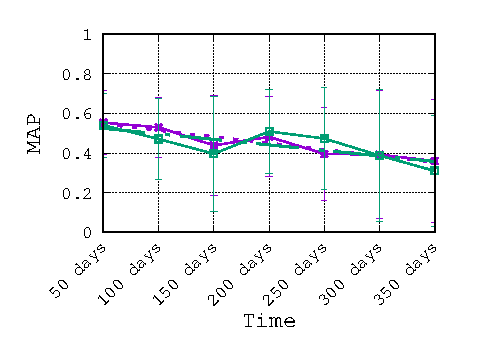
\includegraphics[width=4.9cm]{images/validation_comparaison/average_topics_ap}}
\subfloat[Fig:][]{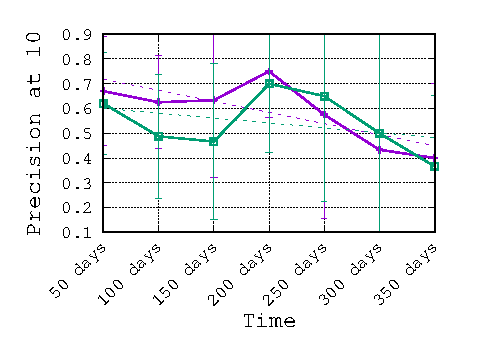
\includegraphics[width=4.9cm]{images/validation_comparaison/average_topics_p10}}
\subfloat[Fig:][]{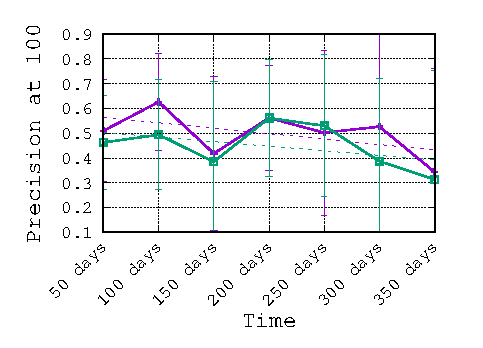
\includegraphics[width=4.9cm]{images/validation_comparaison/average_topics_p100}}
\par\end{centering}
\begin{centering}
\subfloat[Fig:][]{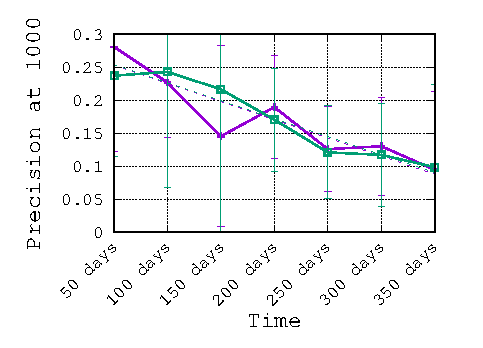
\includegraphics[width=4.9cm]{images/validation_comparaison/average_topics_p1000}}
\subfloat[Fig:][]{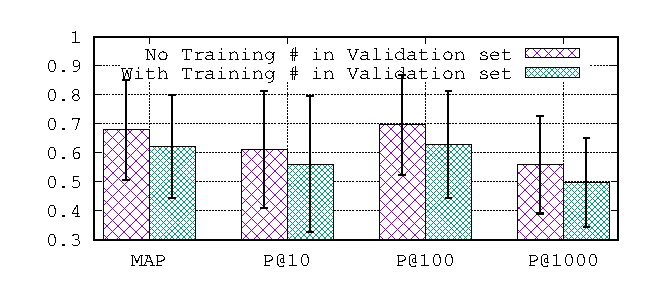
\includegraphics[width=9cm]{images/validation_comparaison/average_topics.eps}}
\par\end{centering}
\caption{Performance obtained while tunning hyperparameters using validation sets with/without tweets containing training hashtags.}
\label{fig:ClassifiersRobustness}
\end{figure}


\textcolor{red}{
\begin{itemize}
    \item Over time,  it is clear that the classification performance drops -- roughly 35\% drop in Mean Average Precision after 350 days of training, which is a significant decrease. We impute this  to the fact that over long periods of time, features that are predictive during the training period may  prove ephemeral and fail to generalize to prediction at future times. This clearly suggests that for such a temporal topic classification, it is necessary to retrain the model after a short period of time to keep a reasonable prediction performance.
    \item Although simple, our approach to avoid overfitting due the problem mentionned above  allows to get roughly 11\% improvement for Means Average  Precision as shown in Figure~\ref{fig:ClassifiersRobustness} (e). Also, while not statistically significant, the linear regression lines suggest that there may be a long-term generalization advantage to excluding training hashtags from the validation data used for hyperparameter tuning.
\end{itemize}
}

\textcolor{red}{In the next section we  report and discuss the main results of the experimental evaluation regarding our interpretation of which features are valuable in classification.}

% Preview source code for paragraph 1




%Having cases of topical tweets not being correctly labeled as topical,
%provides evidence that our method of labeling tweets has limitations
%and our MAP and P@$n$ values are in fact suffering from this
%problem. However, this shows the power of Logistic Regression method
%in generalizing from a small set of hashtags.




\subsection*{Feature Analysis}
\label{label:featureanalysis}

In this section, we analyze the informativeness of feature sets defined in the Data Description section and the effect of their
attributes on learning targeted topical classifiers. To this end,
our goal in this section is to answer the following questions:
\begin{itemize}
\item What are the best features for learning classifiers and do they differ by topic?
\item For each feature type, do any attributes correlate with importance?
\end{itemize}

To answer these questions, we use Mutual Information (MI) (\cite{manning_ir}) as our primary
metric for feature evaluation.  Mutual Information is a general method
for measuring the amount of information one random variable contains
about another random variable and is used to select
predictive features in machine learning.  To calculate the amount of
information that each feature
$j \in \{ \textit{User} \cup \textit{Hashtag} \cup \textit{Mention} \cup \textit{Term} \cup \textit{Location} \}$
provides w.r.t.\ each topic label $t \in \{$Natural Disaster, Epidemics $,\cdots\}$,
Mutual Information is formally defined as:
\begin{align*}
I(j, t) & = \!\!\! \sum_{t \in \{ \mathrm{0}, \mathrm{1} \}} \sum_{j \in \{ \mathrm{0}, \mathrm{1}\}}p(j,t)\log \left ( \frac{p(j,t)}{p(j)p(t)} \right ) 
 \label{eq:eq1}
\end{align*}
with marginal probabilities of topic $p(t)$ and feature $p(j)$ occurrence and joint probability $p(t,j)$ computed over the sample space of all tweets, 
where higher values for this metric indicate more informative features $j$ for the topic $t$.




\begin{figure}[t!]
\centering
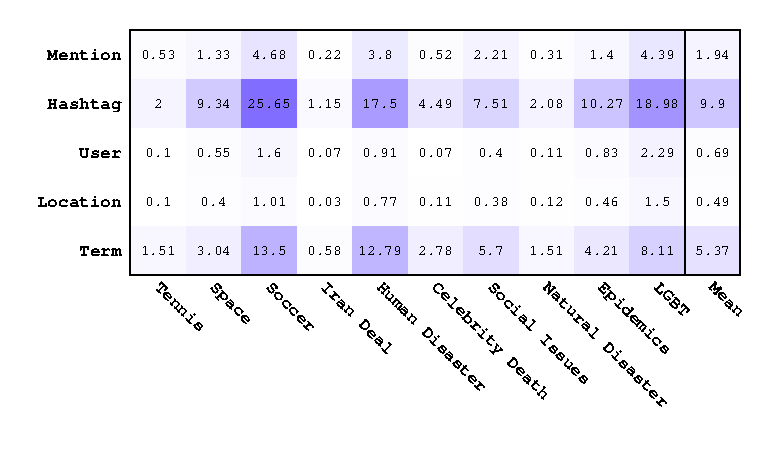
\includegraphics[width=0.8\textwidth]{images/avgMI_gray}
\caption{Matrix of mean Mutual Information values for different feature types vs. topics.  The last column and last row represent the average of mean values across all topics and all features respectively.  All values should be multiplied by $10^{-8}$.)}
\label{fig:avgMI}
\end{figure}

\begin{figure}[t!]
\centering
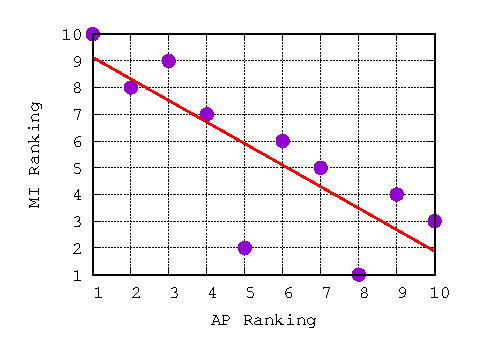
\includegraphics[width=0.4\textwidth]{images/ap_mi_correlation_ranking}
\caption{Scatter plot showing ranking of topics w.r.t. Mutual Information vs. Average Precision. There is clearly a negative correlation, with a Kendall $\tau$ coefficient of $-0.68$.}
\label{fig:ap_mi_correlation_ranking}
\end{figure}


In order to answer the first question regarding the best features
for learning topical classifiers, we provide the mean Mutual Information
values for each feature across different topics in Figure~\ref{fig:avgMI}.
The last column in Figure~\ref{fig:avgMI} shows the
average of the mean Mutual Information for each feature type. \textcolor{red}{ The last row in Figure~\ref{fig:avgMI} shows the
average of the mean Mutual Information for each topic.} From analysis of
Figure~\ref{fig:avgMI}, we can make a set of observations:
\begin{itemize}
\item The \textit{Hashtag} and \textit{Term} features are the most informative features on average. \textcolor{red}{ \textit{Hashtags} are commonly used on Twitter to tag topics of interest associated with a given post, which explains their high informativness.}

% and in general, the more features you have, the better the chance that one is useful.

\item  \textcolor{red}{We note that ranking of topics based on MI is: \emph{Soccer, Human Disaster, LGBT, Epidemics, Social Issue, Space, Celebrity Death, Tennis, Natural Disaster, Iran.}}

\item \textcolor{red}{The topics \textit{Iran Nuclear Deal}, \textit{Tennis} and \textit{Natural Disasters} have low overall features correlation based on Mutual Information. However, these topics  are in the list of top MAP scores using the \textit{Logistic Regression} classifier. In Figure~\ref{fig:ap_mi_correlation_ranking} we shown a scatterplot of the topics ranked by Mutual Information vs. Average Precision. Clearly, we observe that there is a negative topic ranking correlation between the ranking based on AP and MI. The Kendall $\tau$  rank correlation coefficient is $-0.68$, which a relatively high negative value. We explain this negative correlation by the facts that: (i) low MI values doesn't mean that the features are not predictive. (ii) Moreover, during the hyper-parameter validation step, low MI values, in general, will force the process to select fewer features for training a model that will be used for making predictions on the test set. Hence, selecting few features  induces a more robust classifier to overfitting. However, high MI values will force the validation process to select more features for training the model -- they can be good on the validation set for short term prediction, which may fail to generalize for making prediction over long period of time.}

\item The Location feature provides the highest MI regarding the topics of \textit{Human Disaster}, \textit{LBGT}, and \textit{Soccer} indicating a lot of content in these topics is heavily localized. 


\item \textcolor{red}{ Looking at the overall average values, the order of informativeness of feature types appears to be the following: \textit{Hashtag}, \textit{Term}, \textit{Mention}, \textit{User}, \textit{Location}.}
\end{itemize}




\begin{figure*}[tp!]
\centering
\begin{tabular}{ccccc}
%\fbox{\rule{10cm}{3.85cm}}
\subfloat[Fig:][Tennis.]{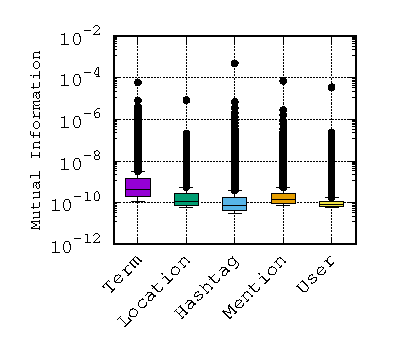
\includegraphics[width=0.20\textwidth]{images/avgMIBoxPlots/Tennis_features.eps}}
\subfloat[Fig:][Space.]{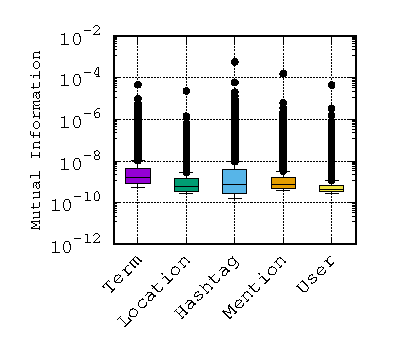
\includegraphics[width=0.20\textwidth]{images/avgMIBoxPlots/Space_features.eps}}
\subfloat[Fig:][Soccer.]{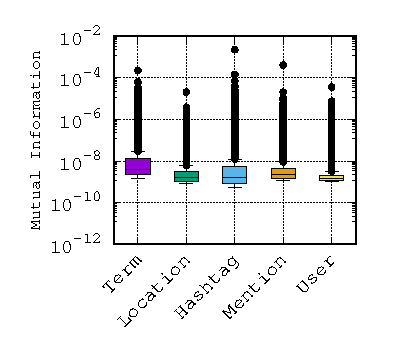
\includegraphics[width=0.20\textwidth]{images/avgMIBoxPlots/Soccer_features.eps}}
\subfloat[Fig:][Iran Nuclear Deal.]{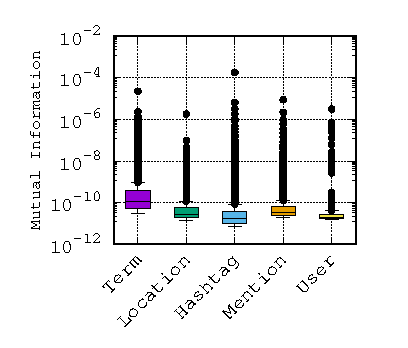
\includegraphics[width=0.20\textwidth]{images/avgMIBoxPlots/Iran_features.eps}}
\subfloat[Fig:][Human Disaster.]{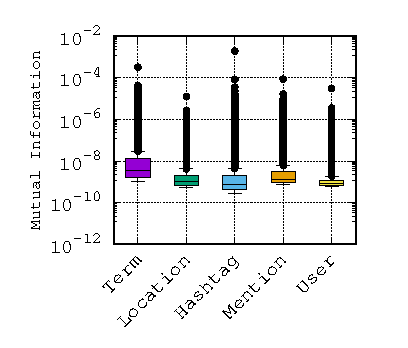
\includegraphics[width=0.20\textwidth]{images/avgMIBoxPlots/Human_Disaster_features.eps}} \\
\subfloat[Fig:][Celebrity Death.]{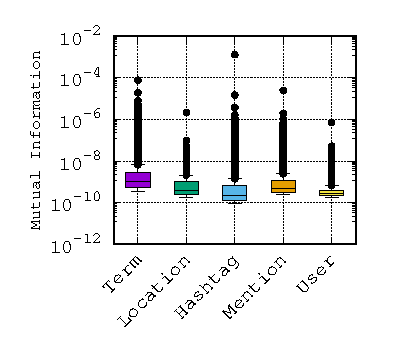
\includegraphics[width=0.20\textwidth]{images/avgMIBoxPlots/Cele_death_features.eps}}
\subfloat[Fig:][Social Issue.]{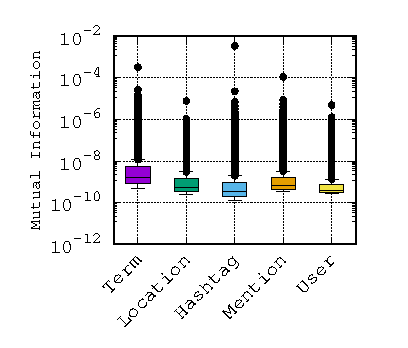
\includegraphics[width=0.20\textwidth]{images/avgMIBoxPlots/Social_issue_features.eps}}
\subfloat[Fig:][Natural Disaster.]{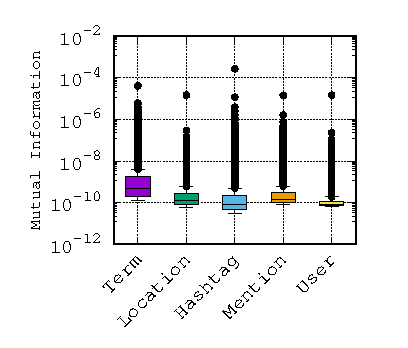
\includegraphics[width=0.20\textwidth]{images/avgMIBoxPlots/Natr_Disaster_features.eps}}
\subfloat[Fig:][Epidemics.]{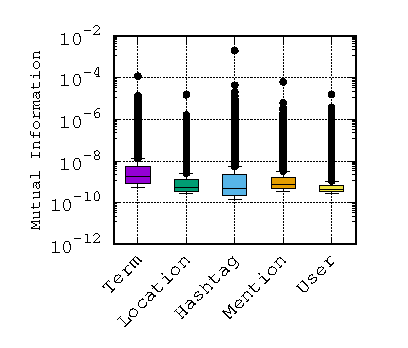
\includegraphics[width=0.20\textwidth]{images/avgMIBoxPlots/Health_features.eps}}
\subfloat[Fig:][LGBT.]{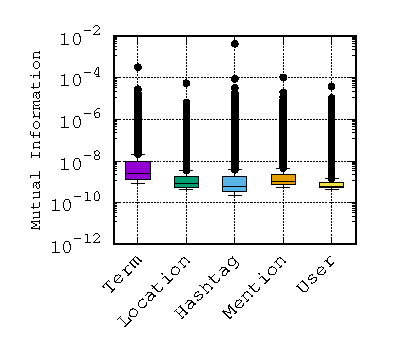
\includegraphics[width=0.20\textwidth]{images/avgMIBoxPlots/LGBT_features.eps}}
\end{tabular}
%\vspace{-2mm}
\caption {Box plots of Mutual Information values (y-axis) per feature type across topics (x-axis labels).}
\label{fig:avgMIBP}
\vspace{2mm}
\end{figure*}


\begin{figure*}[t!]
\centering
\begin{tabular}{ccccc}
%\fbox{\rule{10cm}{3.85cm}}

\includegraphics[width=0.9\textwidth]{images/StackedHistos/legend2.eps}\\
\subfloat[Fig:][Tennis.]{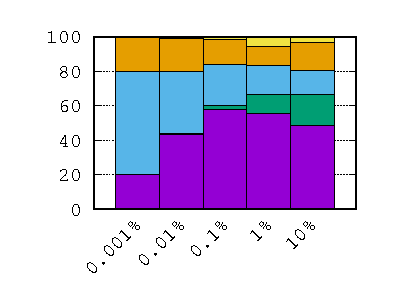
\includegraphics[width=0.20\textwidth]{images/StackedHistos/Tennis_stacked_histo.eps}}
\subfloat[Fig:][Space.]{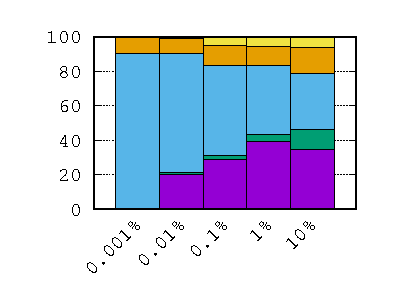
\includegraphics[width=0.20\textwidth]{images/StackedHistos/Space_stacked_histo.eps}}
\subfloat[Fig:][Soccer.]{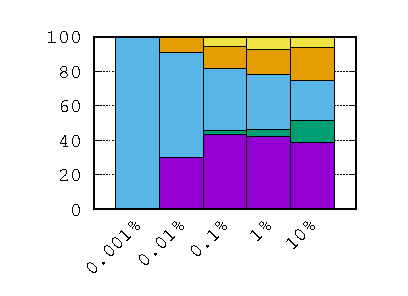
\includegraphics[width=0.20\textwidth]{images/StackedHistos/Soccer_stacked_histo.eps}}
\subfloat[Fig:][Iran Nuclear Deal.]{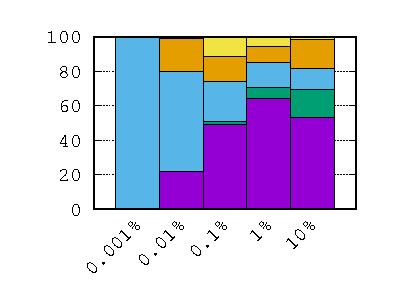
\includegraphics[width=0.20\textwidth]{images/StackedHistos/Iran_stacked_histo.eps}}
\subfloat[Fig:][Human Disaster.]{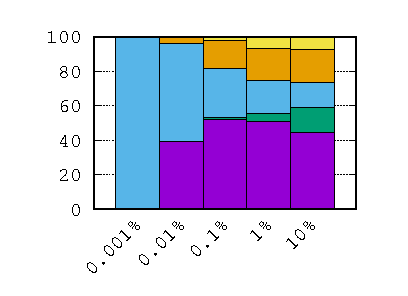
\includegraphics[width=0.20\textwidth]{images/StackedHistos/Human_Disaster_stacked_histo.eps}} \\
\subfloat[Fig:][Celebrity Death.]{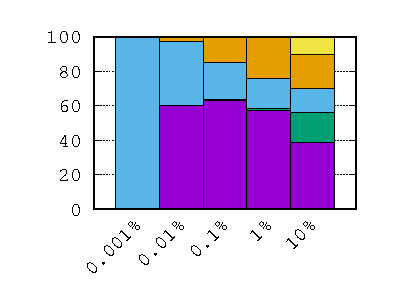
\includegraphics[width=0.20\textwidth]{images/StackedHistos/Cele_death_stacked_histo.eps}}
\subfloat[Fig:][Social Issue.]{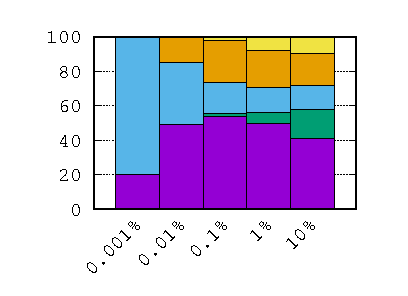
\includegraphics[width=0.20\textwidth]{images/StackedHistos/Social_issue_stacked_histo.eps}}
\subfloat[Fig:][Natural Disaster.]{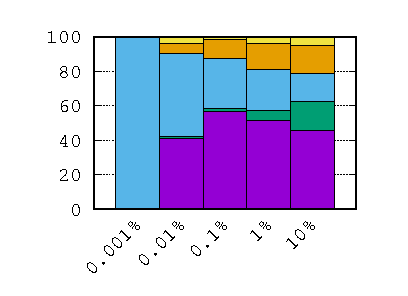
\includegraphics[width=0.20\textwidth]{images/StackedHistos/Natr_Disaster_stacked_histo.eps}}
\subfloat[Fig:][Epidemics.]{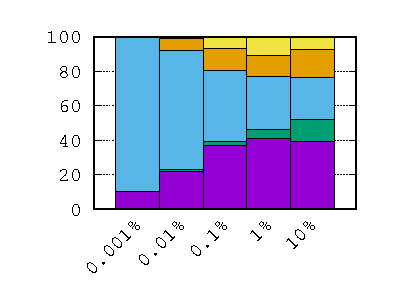
\includegraphics[width=0.20\textwidth]{images/StackedHistos/Health_stacked_histo.eps}}
\subfloat[Fig:][LGBT.]{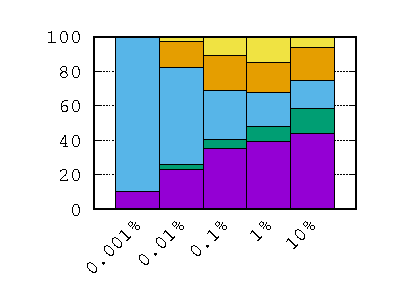
\includegraphics[width=0.20\textwidth]{images/StackedHistos/LGBT_stacked_histo.eps}}
\end{tabular}
%\vspace{-2mm}
\caption {Top $p\%$ features ranked by Mutual Information.}
\label{fig:topMIStacked}
\vspace{2mm}
\end{figure*}






To further analyze the relationship between the informativeness of feature types and topics,
we refer to the box plots of Figure~\ref{fig:avgMIBP}.  Here we see the quartiles and outliers of
the distribution rather than just the average of the MI values in order to ensure the mean MI
values were not misleading our interpretations.  Overall, the story is the same: \textcolor{red}{ hashtag
and term} features dominate in terms of MI followed by the other less informative
features.  \textcolor{red}{Furthermore, three observations are apparent: (1) the topic has little impact on which feature
is most important indicating \emph{stability of feature type informativeness over topics}, (2) hashtags have overall a lower median than terms, locations and mentions, and (3)  hashtags have more outliers indicating that
\emph{the most useful individual features may be terms}. To support this latter claim, we refer to Figure~\ref{fig:topMIStacked}.
Here, we first rank the features according to their MI values and then we consider the top $p\%$ ( $p\% \in \{0.001\%, 0.01\%, 0.1\%, 1\%, 10\%\}$) features to show the distribution of features according to their category using a stacked bar chart for every topic, where every bar corresponds to the $p\%$ bin, having the colors as a map of the feature types (terms, location, hashtag, mention, and user). We clearly observe that for all topic, top features are dominated by hashtags, which explains the fact that the hashtags have the highest mean MI (see Figure~\ref{fig:avgMI}).
}




As anecdotal evidence to inspect which features are most informative, we refer to
Table~\ref{table:top10MItopicsLocations}, which displays the top five feature instances
for each feature type and topic. \textcolor{red}{For example the term \textit{typhoon} is the most correlated feature term with the topic \textit{Natural Disaster}, the official \textit{UNICEF}\footnote{The United Nations Children's Fund (UNICEF) is an organization that aims to provide emergency food and healthcare to children and mothers in developing countries everywhere.} Twitter account (\textit{@unicef}) is the most correlated feature mention with the Human Disaster topic, and the hashtag \textit{\#science} is the most correlated hashtag feature with the topic \textit{Space}.}
Among many remarkable insights in this table, one key aspect we note is that the \emph{terms appear to be the most generic} (and hence most generalizable) features, providing strong intuition as to why these features figure so prominently in terms of their informativeness. \textcolor{red}{
Even though this may contradict the Information Retrieval rationale that specific concepts (high Inverse Document Frequency) are more informative than generic features (low Inverse Document Frequency), in classification rare terms are called noise features (\cite{manning_ir}). 
Specifically,  for temporal machine learning classification, it has been established that specific features (also called Temporally Unstable Features) may prove ephemeral and fail to generalize to prediction at future times (\cite{Wang2019}). }
The top \emph{locations are also highly relevant to most topics} indicating the overall importance of these tweet features for identifying topical tweets.

% \begin{figure*}[tp!]
% \centering
% \begin{tabular}{ccccc}
% %\fbox{\rule{10cm}{3.85cm}}
% \subfloat[Fig:][Term.]{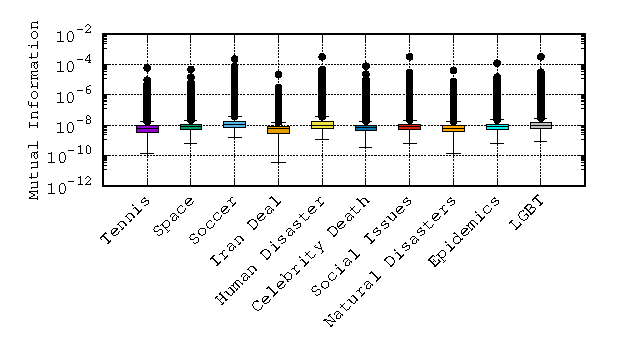
\includegraphics[width=0.34\textwidth]{images/avgMIBoxPlots/term_features}}
% \subfloat[Fig:][Location.]{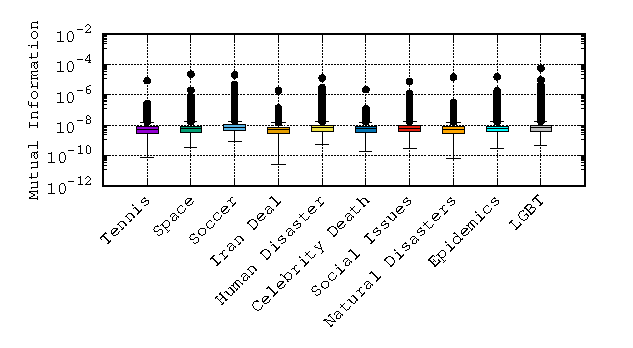
\includegraphics[width=0.34\textwidth]{images/avgMIBoxPlots/loc_features}}
% \subfloat[Fig:][Hashtag.]{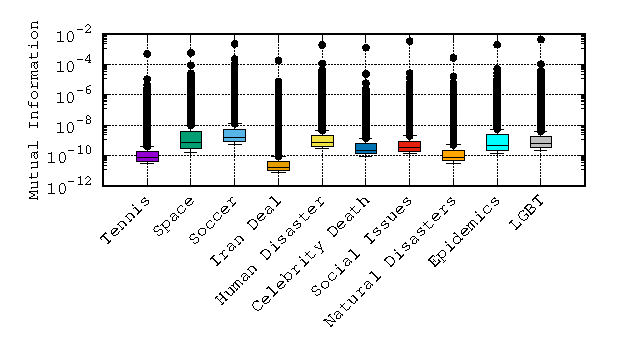
\includegraphics[width=0.34\textwidth]{images/avgMIBoxPlots/hashtag_features}}\\
% \subfloat[Fig:][Mention.]{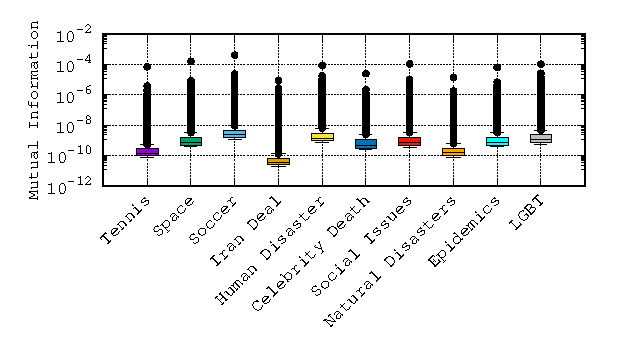
\includegraphics[width=0.33\textwidth]{images/avgMIBoxPlots/mention_features}}
% \subfloat[Fig:][User.]{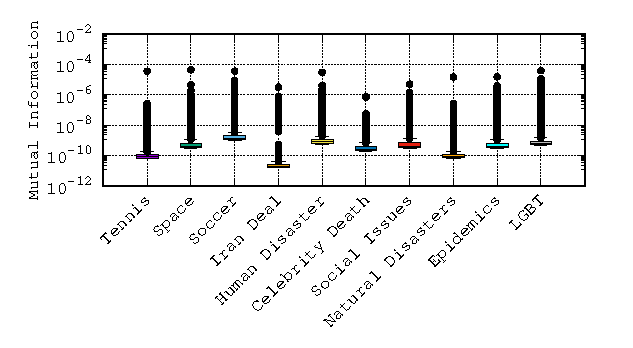
\includegraphics[width=0.33\textwidth]{images/avgMIBoxPlots/user_features}} \\
% \end{tabular}
% %\vspace{-2mm}
% \caption {Box plots of Mutual Information values (y-axis) per feature type across topics (x-axis labels).}
% \label{fig:avgMIBP}
% \vspace{2mm}
% \end{figure*}




\begin{table*}[t!]
\centering
\caption{ The top 5 features for each feature type and topic based on Mutual Information.}
{\renewcommand{\arraystretch}{1.2}
\resizebox{\textwidth}{!}{%
\begin{tabular}{|l|l|l|l|l|l|l|l|l|l|l|}
\hline 
\textbf{Topics/Top10} & \textbf{Natural Disaster} & \textbf{Epidemics} & \textbf{Iran Deal} & \textbf{Social Issues} & \textbf{LBGT} & \textbf{Human Disaster} & \textbf{Celebrity Death} & \textbf{Space} & \textbf{Tennis} & \textbf{Soccer}\tabularnewline
\hline 
\hline 
\textbf{User} & from\_japan & changedecopine & mazandara & debtadvisoruk & stevendickinson & witfp & boiknox & daily\_astrodata & tracktennisnews & makeupbella\tabularnewline
\hline 
\textbf{User} & everyearthquake & stylishoz & freeiran9292 & nsingerdebtpaid & mgdauber & ydumozyf & jacanews & freesolarleads & novakdjokovic\_i & sport\_agent\tabularnewline
\hline 
\textbf{User} & quakestoday & drdaveanddee & hhadi119 & negativeequityf & lileensvf1 & syriatweeten & ewnreporter & sciencewatchout & i\_roger\_federer & yasmingoode\tabularnewline
\hline 
\textbf{User} & equakea & soliant\_schools & balouchn2 & iris\_messenger & kevinwhipp & rk70534 & rowwsupporter & houston\_jobs & andymurrayfans1 & sportsroadhouse\tabularnewline
\hline 
\textbf{User} & davewinfields & msgubot & jeffandsimon & dolphin\_ls & petermabraham & gosyrianews & flykiidchris & lenautilus & rafaelnadal\_fan & losangelessrh\tabularnewline
\hline 
\hline 
\textbf{Hashtag} & \#earthquake & \#health & \#iran & \#ferguson & \#tcot & \#syria & \#rip & \#science & \#wimbledon & \#worldcup\tabularnewline
\hline 
\textbf{Hashtag} & \#haiyan & \#uniteblue & \#irantalks & \#mikebrown & \#pjnet & \#gaza & \#ripcorymonteith & \#sun & \#tennis & \#lfc\tabularnewline
\hline 
\textbf{Hashtag} & \#storm & \#ebola & \#iranian & \#ericgarner & \#p2 & \#israel & \#riprobinwilliams & \#houston & \#usopen & \#football\tabularnewline
\hline 
\textbf{Hashtag} & \#PrayForThePhilippines & \#healthcare & \#rouhani & \#blacklivesmatter & \#uniteblue & \#gazaunderattack & \#rippaulwalker & \#starwars & \#nadal & \#worldcup2014\tabularnewline
\hline 
\textbf{Hashtag} & \#tornado & \#fitness & \#irantalksvienna & \#icantbreathe & \#teaparty & \#isis & \#robinwilliams & \#scifi & \#wimbledon2014 & \#sports\tabularnewline
\hline 
\hline 
\textbf{Location} & With everyone & USA & France & St Louis MO & USA & Syria & South Africa & Houston TX & Worldwide & Liverpool\tabularnewline
\hline 
\textbf{Location} & Earth & Francophone & Tehran Iran & Washington DC & Bordentown New Jersey & Palestine & Pandaquotescom & Germany & London & Manchester\tabularnewline
\hline 
\textbf{Location} & Philippines & United States & Inside of Iran & St Louis & Global Markets & Syrian Arab Republic & Johannesburg South Africa & Houston & The Midlands & London\tabularnewline
\hline 
\textbf{Location} & Don't follow me am i a bot & Gainesville FL USA & Iran & Virginia US & The blue regime of Maryland & Israel & Johannesburg & Rimouski & London UK & Anfield\tabularnewline
\hline 
\textbf{Location} & Global planet earth & Boulder Colorado & Washington DC & Saint Louis MO & Lancaster county PA & Washington DC & Cape Town & In a galaxy far far ebay & Wimbledon & Bangil East Java Indonesia\tabularnewline
\hline 
\hline 
\textbf{Mention} & @oxfamgb & @foxtramedia & @ap & @natedrug & @jjauthor & @ifalasteen & @nelsonmandela & @nasa & @wimbledon & @lfc\tabularnewline
\hline 
\textbf{Mention} & @gabriele\_corno & @obi\_obadike & @afp & @deray & @2anow & @drbasselabuward & @realpaulwalker & @philae2014 & @usopen & @fifaworldcup\tabularnewline
\hline 
\textbf{Mention} & @weatherchannel & @who & @iran\_policy & @antoniofrench & @gop & @revolutionsyria & @ddlovato & @maximaxoo & @atpworldtour & @ussoccer\tabularnewline
\hline 
\textbf{Mention} & @twcbreaking & @kayla\_itsines & @4freedominiran & @bipartisanism & @pjnet\_blog & @unicef & @robinwilliams & @esa\_rosetta & @andy\_murray & @mcfc\tabularnewline
\hline 
\textbf{Mention} & @redcross & @canproveit & @orgiac & @theanonmessage & @espuelasvox & @free\_media\_hub & @historicalpics & @astro\_reid & @wta & @realmadriden\tabularnewline
\hline 
\hline 
\textbf{Term} & typhoon & health & nuclear & police & obama & israeli & robin & space & tennis & liverpool\tabularnewline
\hline 
\textbf{Term} & philippines & ebola & regime & protesters & gun & israel & williams & solar & murray & cup\tabularnewline
\hline 
\textbf{Term} & magnitude & outbreak & iran & officer & america & gaza & walker & moon & djokovic & supporting\tabularnewline
\hline 
\textbf{Term} & storm & virus & iranian  & cops & obamacare & palestinian & cory & houston & federer & match\tabularnewline
\hline 
\textbf{Term} & usgs & acrx & mullahs & protest & gop & killed & paul & star & nadal & goal\tabularnewline
\hline 
\end{tabular}

}}
\label{table:top10MItopicsLocations}
\end{table*}







% Need more insight than this! -SPS
%
%It can be observed that the different locations, hashtags, or terms
%shown as the top features based on Mutual Information are actually in
%relation with the specific topic.

In order to answer the second question on whether any attributes
correlate with importance for each feature, we provide two types of
analysis \textcolor{red}{using the topic \textit{Celebrity Death} -- 
the other topics showed similar patterns, thus we have chosen to omit them.} 
The first analysis shown in Figure~\ref{fig:violinplots}
analyzes the distributions of Mutual Information values for features
when binned by the magnitude of various attributes of those
features, outlined as follows:
\begin{itemize}
\item \textbf{From} vs. 
\begin{itemize}
\item \textit{Favorite count:} \# of tweets user has favorited.
\item \textit{Followers count:} \# of users who follow user.
\item \textit{Friends count:} \# of users followed by user.
\item \textit{Hashtag count:} \# of hashtags used by user.
\item \textit{Tweet count:} \# of tweets from user.
 \end{itemize}
\end{itemize}
\begin{itemize}
\item \textbf{Hashtag} vs.
\begin{itemize}
\item \textit{Tweet count:} \# of tweets using hashtag.
\item \textit{User count:} \# of users using hashtag.
\end{itemize}
\end{itemize}
\begin{itemize}
\item \textbf{Location} vs. \textit{User count:} \# of users using location.
\item \textbf{Mention} vs. \textit{Tweet count:} \# of tweets using mention.
\item \textbf{Term} vs. \textit{Tweet count:} \# of tweets using term.
\end{itemize}

As we can see in the boxplots of Figure~\ref{fig:violinplots}, the
general pattern is that the greater the number of tweets, users, or
hashtag count a feature has, the more informative the feature is in general.
This pattern also exists to some extent on the attributes
of the \textit{From} feature, although the pattern is less visible in
general and not clear (or very weak) for the follower or friend count.
In general, the informativeness of a user appears to have little correlation
with their follower or friend count.

\textcolor{red}{Figure~\ref{fig:densityplots} provides a further analysis by showing
density plots of the tweet count attribute  of the \textit{User}, \textit{Hashtag},
\textit{Mention} and \textit{Term}  features, and the user count attribute of 
the \textit{Hashtag} feature. Here we can clearly observe the positive linear correlation
that exists between the attribute magnitude and the Mutual Information value.
}
%Here we see an
%interesting phenomenon that was not clear in the Violin plots: there
%is a very clear bimodality of the density.  On further investigation
%it turns out that the top mode feature occurs in at least one topical
%tweet whereas the bottom mode occurs in no topical tweets.  While the
%bottom mode features may serve as good indicators of non-topicality,
%the top mode are inherently more indicative of topicality, which
%justifies feature selection by mutual information.



\begin{figure*}[tp!]
\centering
\begin{tabular}{ccccc}
\begin{tabular}{ccccc} % height=35mm -- always scale graphics proportionally by just specifying one dim. -SPS
\subfloat[Fig:][ User \# of favorites.]{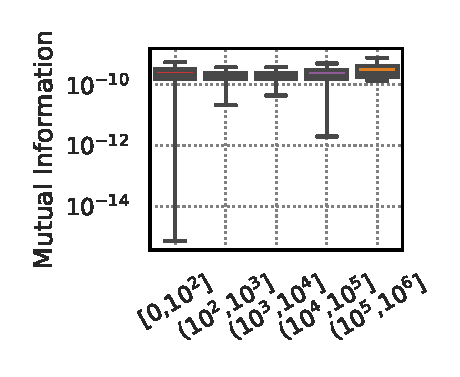
\includegraphics[width=0.20\textwidth]{images/BoxPlots_Cele_death/Cele_death_user_favouritesCount_boxplots.eps}}
\subfloat[Fig:][User \# of followers.]{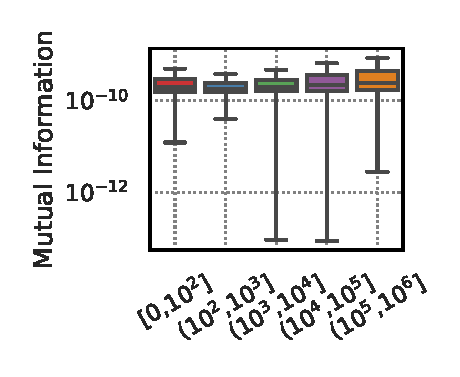
\includegraphics[width=0.20\textwidth]{images/BoxPlots_Cele_death/Cele_death_user_followersCount_boxplots.eps}}
\subfloat[Fig:][User \# of friends.]{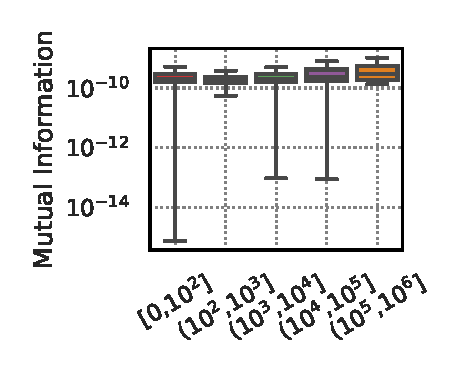
\includegraphics[width=0.20\textwidth]{images/BoxPlots_Cele_death/Cele_death_user_friendsCount_boxplots.eps}}
\subfloat[Fig:][User \# of hashtags.]{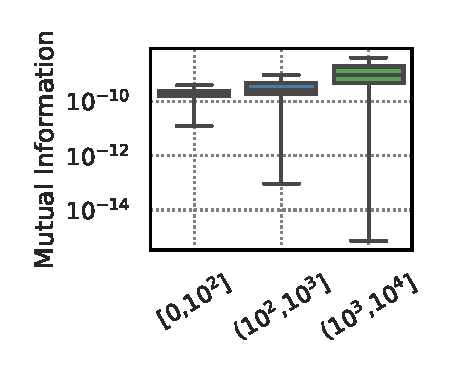
\includegraphics[width=0.20\textwidth]{images/BoxPlots_Cele_death/Cele_death_user_hashtagCount_boxplots.eps}}
\subfloat[Fig:][User \# of tweets.]{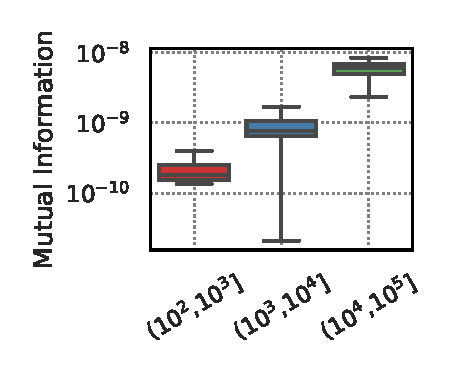
\includegraphics[width=0.20\textwidth]{images/BoxPlots_Cele_death/Cele_death_user_tweetCount_boxplots.eps}} \\
%\vspace{-10mm}
\subfloat[Fig:][Hashtag \# of tweets.]{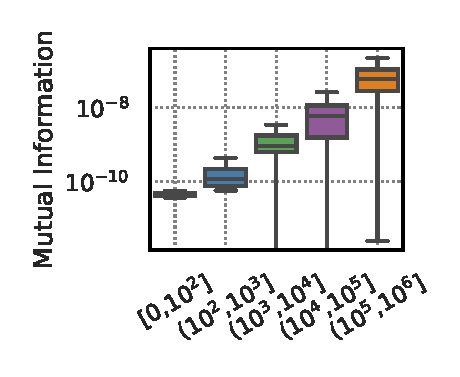
\includegraphics[width=0.20\textwidth]{images/BoxPlots_Cele_death/Cele_death_hashtag_tweetCount_boxplots.eps}}
\subfloat[Fig:][Hashtag \# of users.]{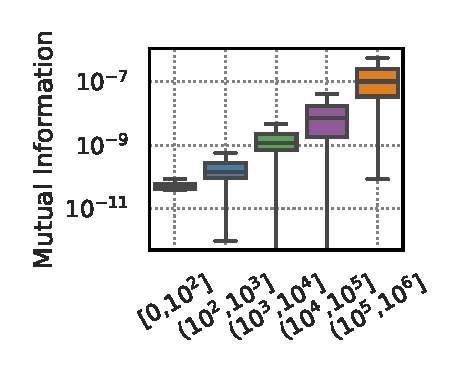
\includegraphics[width=0.20\textwidth]{images/BoxPlots_Cele_death/Cele_death_hashtag_userCount_boxplots.eps}}
\subfloat[Fig:][Location \# of users.]{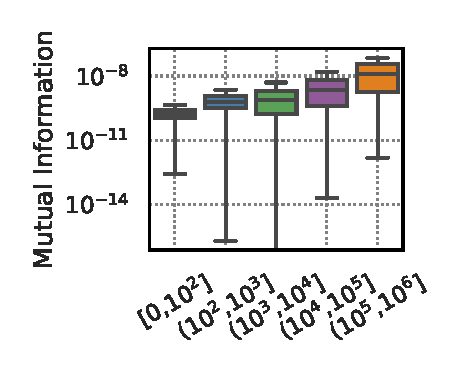
\includegraphics[width=0.20\textwidth]{images/BoxPlots_Cele_death/Cele_death_location_userCount_boxplots.eps}}
\subfloat[Fig:][Mention \# of tweets.]{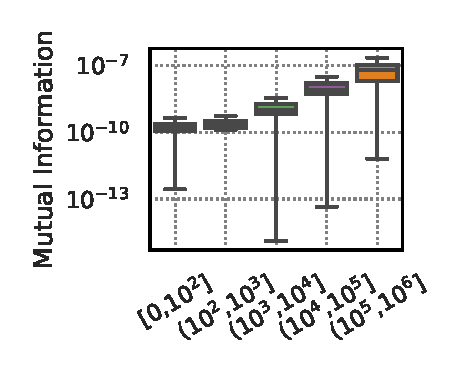
\includegraphics[width=0.20\textwidth]{images/BoxPlots_Cele_death/Cele_death_mention_tweetCount_boxplots.eps}}
\subfloat[Fig:][Term \# of tweets.]{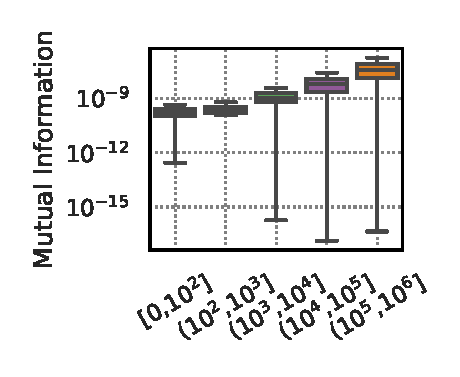
\includegraphics[width=0.20\textwidth]{images/BoxPlots_Cele_death/Cele_death_term_tweetCount_boxplots.eps}} \\
\end{tabular}
\end{tabular}
%\vspace{-2mm}
\caption {Boxplots for the distribution of Mutual Information values (y-axis) of different features as a function of their attribute values (binned on x-axis).  Plots (a-e) respectively show attributes \{favoriteCount, followerCount, friendCount, hashtagCount, tweetCount\} for \textit{From} feature. Plots (f-j) respectively show attributes tweetCount and userCount for \textit{Hashtag}, userCount for \textit{Location} feature, tweetCount for \textit{Mention} and \textit{Term} features.}
\label{fig:violinplots}
\vspace{2mm}
\end{figure*}

\begin{figure*}[t!]
\centering
\begin{tabular}{cccc} % height=35mm -- always scale graphics proportionally by just specifying one dim. -SPS
\subfloat[Fig:][]{\includegraphics[width=0.20\textwidth]{images/DensityPlots_Cele_death/Cele_death_user_tweetCount_scatter.eps}}
\subfloat[Fig:][]{\includegraphics[width=0.20\textwidth]{images/DensityPlots_Cele_death/Cele_death_hashtag_tweetCount_scatter.eps}}
\subfloat[Fig:][]{\includegraphics[width=0.20\textwidth]{images/DensityPlots_Cele_death/Cele_death_hashtag_userCount_scatter.eps}} 
\subfloat[Fig:][]{\includegraphics[width=0.20\textwidth]{images/DensityPlots_Cele_death/Cele_death_mention_tweetCount_scatter.eps}} 
\subfloat[Fig:][]{\includegraphics[width=0.20\textwidth]{images/DensityPlots_Cele_death/Cele_death_term_tweetCount_scatter.eps}}
\end{tabular}
\vspace{-2mm}
\caption {Density plots for the frequency values of feature attributes (x-axis) vs. Mutual Information (y-axis).  Plots (a-d) respectively show attributes \{favoriteCount, followerCount, friendCount, hashtagCount\} for the \textit{From} feature.}
\label{fig:densityplots}
\vspace{2mm}
\end{figure*}


\section*{Conclusions}
%!TEX root = main.tex

This work provides a long-term study of topic classifiers on Twitter that further justifies classification-based topical filtering approaches while providing detailed insight into the feature properties most critical for topic classifier performance.
%
%This work fills a major gap in event detection and tracking from
%social media on identifying emerging topics from long-running themes
%with minimal user supervision.  We contribute a novel supervised
%method for training social sensors with minimal user curation by using
%a small seed set of hashtags as topical proxies for automatic
%supervised data labeling.
%The supervised classification and ranking
%methods learn topical content from a large feature space. We train our
%social sensor on known topical content, but tune it on novel topical
%validation content which ensures optimal generalization. The
%experiments are on a corpus of over $800$ million tweets crawled with
%Twitter Search API.
Our results suggest that these learned topical classifiers generalize well
to unseen future topical content over a long time horizon (i.e., one year)
and provide a novel paradigm for the
extraction of high-value content from social media. Furthermore, an
extensive analysis of features and feature attributes across different
topics has revealed key insights including the following two: 
(i) largely independent of
topic, generic terms are the most informative features followed by
topic-specific locations, and (ii) the number of unique hashtags and
tweets by a user correlates more with their informativeness than their
follower or friend count.

Among many interesting directions, future work might evaluate a range of 
topical classifier extensions: (1)
optimizing rankings not only for topicality but also to minimize the
lag-time of novel content identification, (2) optimizing queries for
boolean retrieval oriented APIs such as Twitter, (3) identification of 
long-term temporally stable predictive features, and (4) utilizing
more social network structure as graph-based 
features.  Altogether, we believe these insights will facilitate 
the continued development of effective topical classifiers for Twitter that learn to
identify broad themes of topical information with minimal user
interaction and enhance the overall social media user experience.


\bibliography{biblio}

\end{document}
